\chapter{Nonprompt Background Estimate}
\label{chap:Nonprompt}

In this analysis, the term \emph{real} leptons refers to prompt leptons that originate from the primary interaction, like the decays of vector bosons that are produced via hard collisions. \emph{Fake} leptons refer to non-prompt leptons that are mostly produced in the decays of b-quarks, c-quarks, pions, or from photon conversion. A relatively low ratio of \emph{fake} leptons in a lepton selection is desired and can be achieved by applying stringent isolation requirements and/or an MVA-based lepton identification specifically trained against \emph{fake} leptons. 

Non-prompt backgrounds are defined to be backgrounds with at least one \emph{fake} lepton passing the analysis selection, in this case generally dominated by Drell-Yan and $t\bar{t}$ production. An accurate estimation of non-prompt backgrounds is difficult to achieve through MC modeling. Therefore, a data-driven technique called the $3$D matrix method is used to estimate the non-prompt backgrounds. 

A brief description of the matrix method is given in this section followed by details on it's implementation. In autorefyou can find more information on the generalization of the matrix method to $2$D and $3$D. The appendices also contain a validation of the method and its performance is compared to the results of the fake factor method, another commonly used data-driven technique.
%%%%%%%%%%%%%%%%%%%%%%%%%%%%%%%%%%%%%%%%%%%%%%%%%%%%%%%%%%%%%
%%%%%%%%%%%%%%%%%%%%%%%%%%%%%%%%%%%%%%%%%%%%%%%%%%%%%%%%%%%%%
\section{The Matrix Method}
\label{sec:MM}

The matrix method cite{matrix2012} is a data driven technique used to estimate the fraction of \emph{fake} leptons that pass a given lepton selection, referred to as "\emph{tight}". The \emph{tight} selection usually incorporates tight lepton identification and isolation requirements and should be similar if not exactly the same as lepton selection in the actual analysis. The \emph{loose} selection is obtained by loosening the \emph{tight} selection. The \emph{loose} selection is used as a baseline such that any leptons that pass it will fall into one of the two exclusive categories: \emph{tight} or \emph{not tight}. The matrix method treats \emph{real} and \emph{fake} leptons separately. As a result, \emph{real} and \emph{fake} efficiencies are introduced (see Figure \ref{fig:Matrix_Method}).

 \begin{figure}[tbh!]
 \begin{center}
 \begin{tabular}{c}
 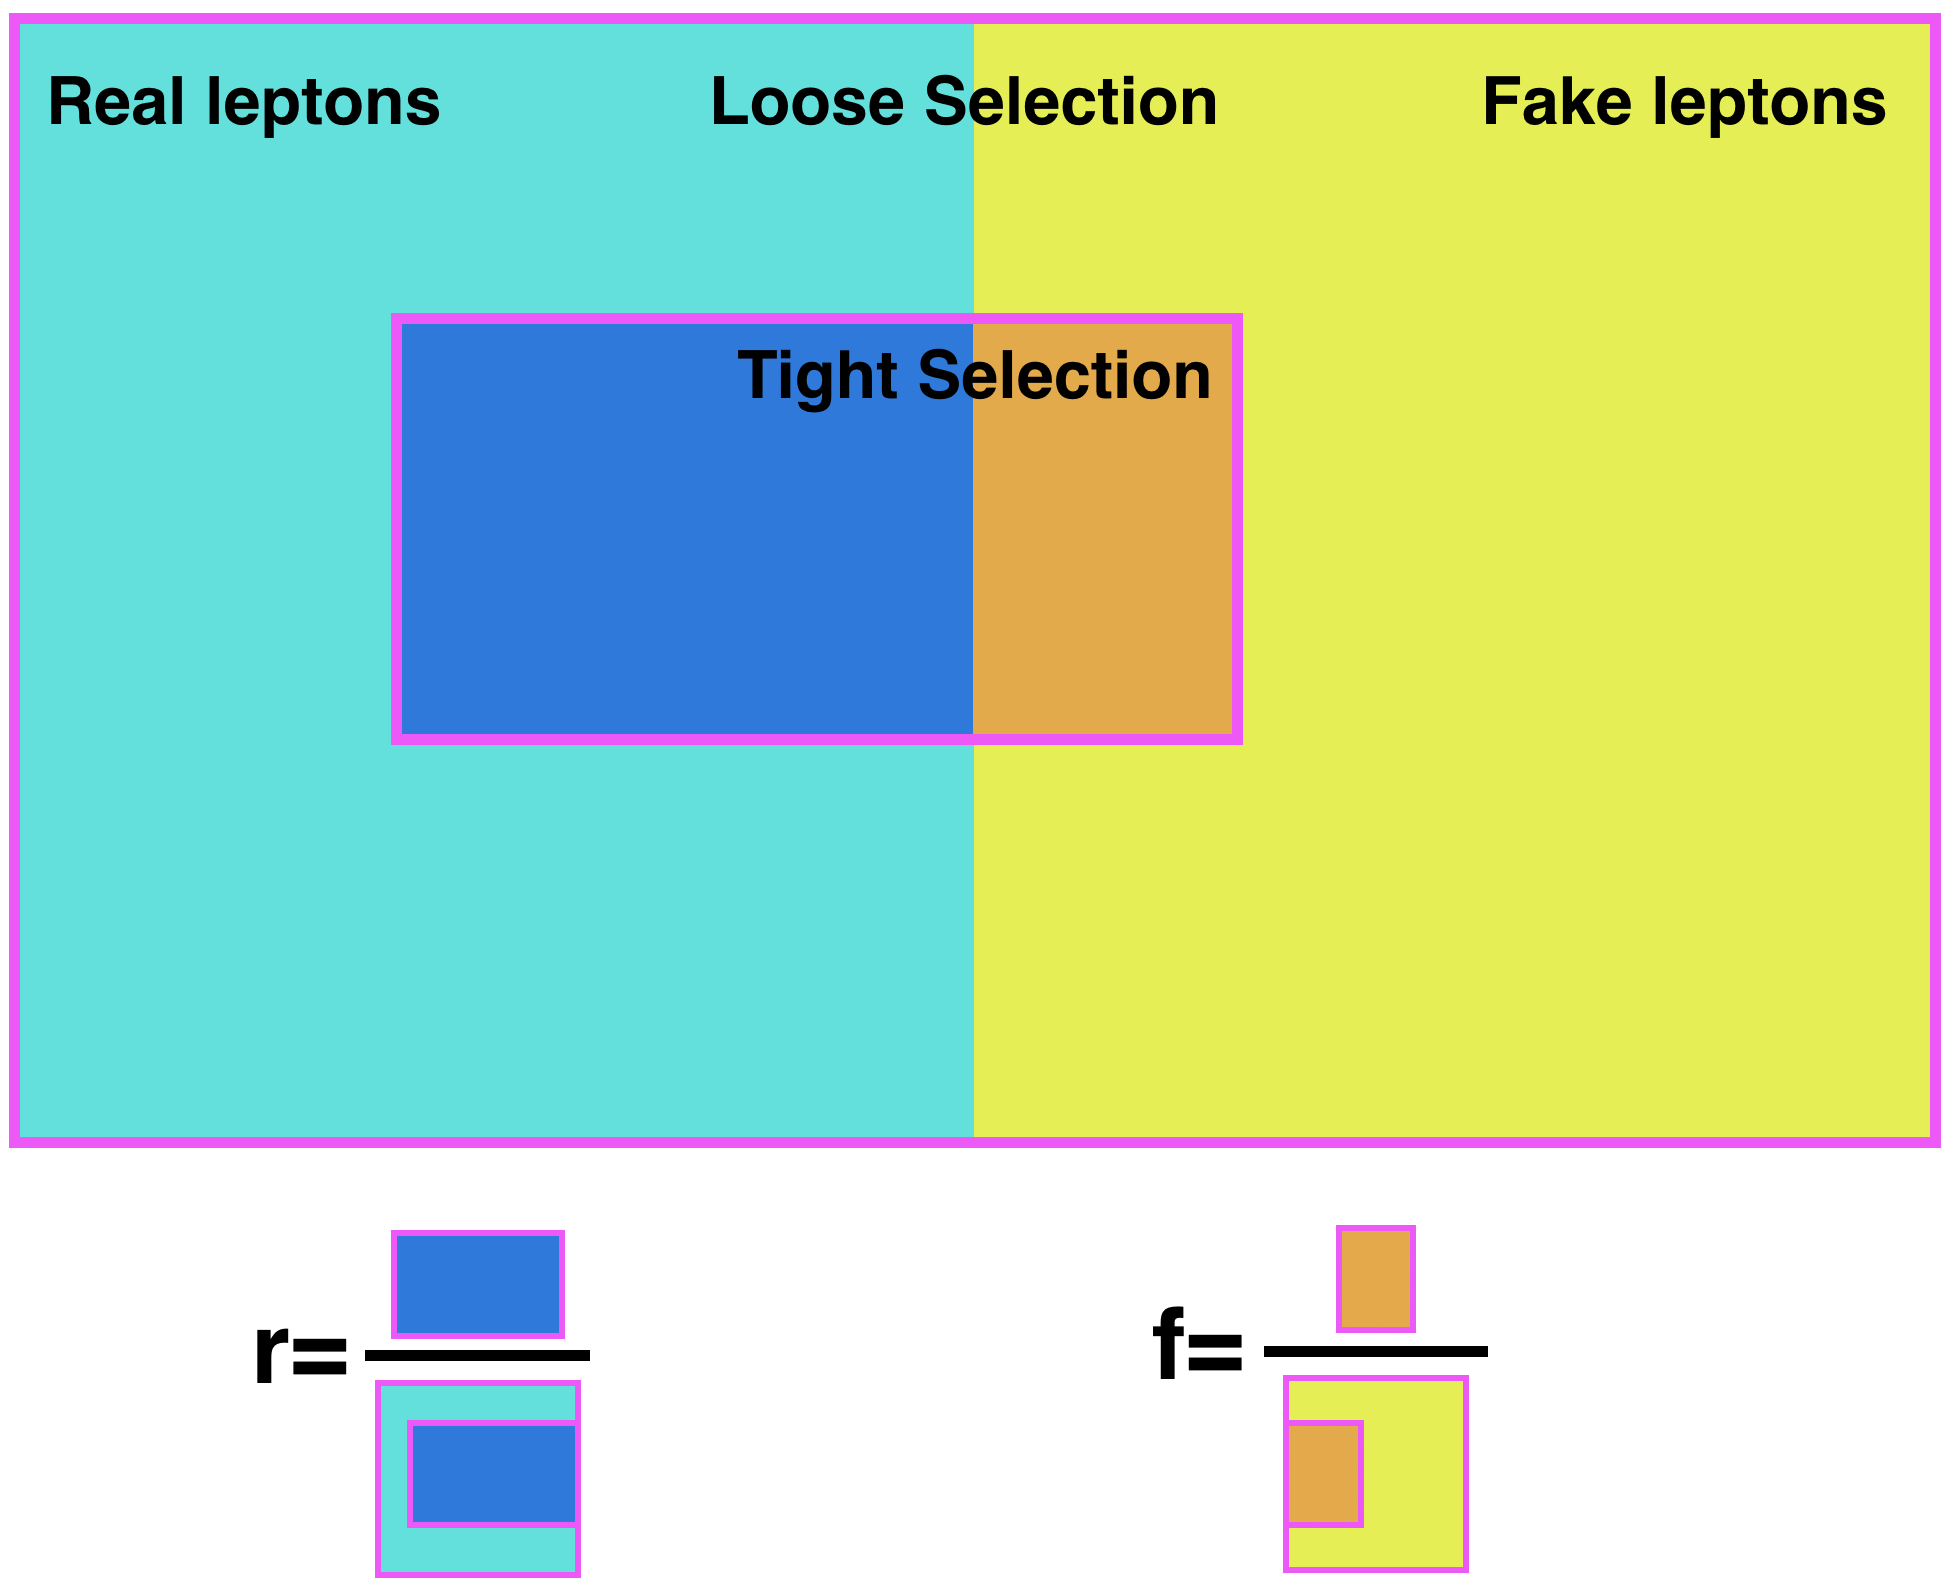
\includegraphics[width=0.7\textwidth]{figures/Part3/Nonprompt/matrix}
 \end{tabular}
 \caption{Illustration of the \emph{real} efficiency $r$ and the \emph{fake} efficiency $f$.}
 \label{fig:Matrix_Method}
 \end{center}
\end{figure}

In a simplified scenario with only one lepton in the final state, the \emph{real} efficiency $r$ measures the likelihood of \emph{real} leptons pass \emph{tight} selection. It is treated as an observable that can be obtained through measurement:
\begin{equation}
r=\frac{n_R^{T}}{n_R^{T}+n_R^{\overline{T}}},
 \label{eq:real_rate}
\end{equation}
in which $n_R^{T}$/$n_R^{\overline{T}}$ denotes the number of events with a \emph{real} lepton that is \emph{tight}/\emph{not tight}.

Similarly, \emph{fake} efficiency $f$ can be expressed as
\begin{equation}
f=\frac{n_F^{T}}{n_F^{T}+n_F^{\overline{T}}},
 \label{eq:fake_rate}
\end{equation}
in which $n_F^{T}$/$n_F^{\overline{T}}$ denotes the number of events with a \emph{fake} lepton that is \emph{tight}/\emph{not tight}.

The measurement of $r/f$ is often performed in dedicated control regions, where high purity of \emph{real}/\emph{fake} leptons is expected. These regions are referred to as the measurement regions (MR). It is assumed that $r/f$ is a universal property of \emph{real}/\emph{fake} leptons that is independent of physics processes. Therefore, $r/f$ extracted from MR can be used to estimate the contamination of \emph{fake} leptons in a different region (e.g. SR) even though these two regions are orthogonal to each other.

In our simplified scenario, the total number of events in the region of interest (e.g. SR/VR) with a \emph{tight}/\emph{not tight} lepton can be expressed in a system of equations:

\begin{equation}
\begin{split}
N^{T}&=N_{R}^{T}+N_{F}^{T}\\
N^{\overline{T}}&=N_{R}^{\overline{T}}+N_{F}^{\overline{T}},
\end{split}
\end{equation}

in which capital letter "N" is used to indicate that these numbers are referring to events in a region that is different from MR. $N_{R}^{\overline{T}}$/$N_{F}^{\overline{T}}$ can be expressed in terms of $r/f$ and $N_{R}^{T}$/$N_{F}^{T}$ according to Equation \ref{eq:real_rate}/\ref{eq:fake_rate} and the assumption that r/f is transferable to other regions:

\begin{equation}
\begin{split}
N^{T}&=r\frac{N_{R}^{T}}{r}+f\frac{N_{F}^{T}}{f}\\
N^{\overline{T}}&=(1-r)\frac{N_{R}^{T}}{r}+(1-f)\frac{N_{F}^{T}}{f}.
\end{split}
\label{eq:sys_eq}
\end{equation}

Equation \ref{eq:sys_eq} can also be expressed in the form of matrix:

\begin{equation}
 \begin{pmatrix}
 N^{T}\\
 N^{\overline{T}}
 \end{pmatrix}=\begin{pmatrix}
r&f\\
1-r&1-f
 \end{pmatrix}\begin{pmatrix}
 N_{R}^{T}/r\\
 N_{F}^{T}/f
 \end{pmatrix}.
 \label{eq:matrix}
 \end{equation}
 
Since those two numbers that appear on the lefthand side of the equation can be obtained through measurement, a matrix inversion can give us an estimation of \emph{fake} leptons that pass \emph{tight} selection, denoted by $N_{F}^T$.
%%%%%%%%%%%%%%%%%%%%%%%%%%%%%%%%%%%%%%%%%%%%%%%%%%%%%%%%%%%%%
%%%%%%%%%%%%%%%%%%%%%%%%%%%%%%%%%%%%%%%%%%%%%%%%%%%%%%%%%%%%%
\section{Extraction of Prompt and Nonprompt Efficiencies}
\label{sec:MR}

The description in previous section deals with a scenario where only one lepton is studied. This analysis uses a generalized version of the matrix method (i.e. 3D matrix method. See autoref{sec:appendixnonprompt} for more details), where all three leptons are considered to be possibly \emph{fake}.

\begin{table}[htbp]
 \begin{center}
 \caption{Parent datasets (2016) used to generate TOP PAG NanoAOD-v6 samples used for $r$ and $f$ measurement. (\small{X = "SingleElectron" and "SingleMuon".)
 }}
 \label{tab:2016_RandF_Samples}
 \begin{tabular}{c|c|c}
  \hline
  & Data type & Samples  \\  
  \hline\hline
  \multirow{20}{*}{$f$} & \multirow{7}{*}{data} &
  /X/Run2016B-17Jul2018\_ver2-v1/MINIAOD \\
  & & /X/Run2016C-17Jul2018-v1/MINIAOD \\
  & & /X/Run2016D-17Jul2018-v1/MINIAOD \\
  & & /X/Run2016E-17Jul2018-v2/MINIAOD \\
  & & /X/Run2016F-17Jul2018-v1/MINIAOD \\
  & & /X/Run2016G-17Jul2018-v1/MINIAOD \\
  & & /X/Run2016H-17Jul2018-v1/MINIAOD \\ \cline{2-3}
  & \multirow{13}{*}{MC} &
  /WZTo3LNu\_TuneCUETP8M1\_13TeV-amcatnloFXFX-pythia8 \\
  & & /ZZTo4L\_13TeV\_powheg\_pythia8 \\
  & & /ttHToNonbb\_M125\_TuneCUETP8M2\_ttHtranche3\_13TeV-powheg-pythia8\\
  & & /TTZToLLNuNu\_M-10\_TuneCUETP8M1\_13TeV-amcatnlo-pythia8 \\
  & & /TTZToLL\_M-1to10\_TuneCUETP8M1\_13TeV-madgraphMLM-pythia8\\
  & & /THQ\_Hincl\_13TeV-madgraph-pythia8\_TuneCUETP8M1   \\
  & & /THW\_Hincl\_13TeV-madgraph-pythia8\_TuneCUETP8M1  \\
  & &/WWW\_4F\_TuneCUETP8M1\_13TeV-amcatnlo-pythia8  \\
  & &/WWZ\_TuneCUETP8M1\_13TeV-amcatnlo-pythia8 \\
  & &/WZZ\_TuneCUETP8M1\_13TeV-amcatnlo-pythia8  \\
  & &/ZZZ\_TuneCUETP8M1\_13TeV-amcatnlo-pythia8  \\
  & & /tZq\_ll\_4f\_ckm\_NLO\_TuneCP5\_PSweights\_13TeV-amcatnlo-pythia8 \\
  & & /TTWJetsToLNu\_TuneCUETP8M1\_13TeV-amcatnloFXFX-madspin-pythia8 \\ \hline
  $r$ & MC & /TTTo2L2Nu\_TuneCUETP8M2\_ttHtranche3\_13TeV-powheg-pythia8 \\ \hline
 \end{tabular}
 \end{center}
\end{table}

\begin{table}[htbp]
 \begin{center}
 \caption{Parent datasets (2017) used to generate TOP PAG NanoAOD-v6 samples used for $r$ and $f$ measurement. (\small{X = "SingleElectron" and "SingleMuon".)
 }}
 \label{tab:2017_RandF_Samples}
 \begin{tabular}{c|c|c}
  \hline
  & Data type & Samples  \\  
  \hline\hline
  \multirow{18}{*}{$f$} & \multirow{5}{*}{data} &
  /X/Run2017B-31Mar2018-v1/MINIAOD \\
  & &/X/Run2017C-31Mar2018-v1/MINIAOD \\
  & & /X/Run2017D-31Mar2018-v1/MINIAOD \\
  & &/X/Run2017E-31Mar2018-v1/MINIAOD \\
  & &/X/Run2017F-31Mar2018-v1/MINIAOD \\ \cline{2-3}
  & \multirow{13}{*}{MC} &
  /WZTo3LNu\_TuneCP5\_13TeV-amcatnloFXFX-pythia8 \\
  & & /ZZTo4L\_13TeV\_powheg\_pythia8 \\
  & & /ttHToNonbb\_M125\_TuneCP5\_13TeV-powheg-pythia8\\
  & & /TTZToLLNuNu\_M-10\_TuneCP5\_13TeV-amcatnlo-pythia8 \\
  & & /WWW\_4F\_TuneCP5\_13TeV-amcatnlo-pythia8 \\
  & & /WWZ\_4F\_TuneCP5\_13TeV-amcatnlo-pythia8 \\
  & & /WZZ\_TuneCP5\_13TeV-amcatnlo-pythia8 \\
  & & /ZZZ\_TuneCP5\_13TeV-amcatnlo-pythia8 \\ 
  & &/TTZToLL\_M-1to10\_TuneCP5\_13TeV-amcatnlo-pythia8 \\
  & & /THQ\_4f\_Hincl\_13TeV\_madgraph\_pythia8 \\
  & & /THW\_5f\_Hincl\_13TeV\_madgraph\_pythia8 \\
  & & /tZq\_ll\_4f\_ckm\_NLO\_TuneCP5\_PSweights\_13TeV-amcatnlo-pythia8 \\
  & & /TTWJetsToLNu\_TuneCP5\_13TeV-amcatnloFXFX-madspin-pythia8 \\ \hline
  $r$ & MC& /TTTo2L2Nu\_TuneCP5\_13TeV-powheg-pythia8 \\ \hline
 \end{tabular}
 \end{center}
\end{table}

\begin{table}[htbp]
\sffamily
 \begin{center}
 \caption{Parent datasets (2018) used to generate TOP PAG NanoAOD-v6 samples used for $r$ and $f$ measurement. (\small{X = "Egamma" and "SingleMuon".)
 }}
 \label{tab:2018_RandF_Samples}
 \begin{tabular}{c|c|c}
  \hline
  & Data type & Samples  \\  
  \hline\hline
  \multirow{17}{*}{$f$} & \multirow{4}{*}{data} &
  /X/Run2018A-17Sep2018-v1/MINIAOD \\
  & &/X/Run2018B-17Sep2018-v1/MINIAOD \\
  & &/X/Run2018C-17Sep2018-v1/MINIAOD \\
  & &/X/Run2018D-PromptReco-v2/MINIAOD \\ \cline{2-3}
  & \multirow{13}{*}{MC} &
  /WZTo3LNu\_TuneCP5\_13TeV-amcatnloFXFX-pythia8 \\
  & & /ZZTo4L\_13TeV\_powheg\_pythia8 \\
  & & /ttHToNonbb\_M125\_TuneCP5\_13TeV-powheg-pythia8\\
  & & /TTZToLLNuNu\_M-10\_TuneCP5\_13TeV-amcatnlo-pythia8 \\
  & & /WWW\_4F\_TuneCP5\_13TeV-amcatnlo-pythia8 \\
  & & /WWZ\_4F\_TuneCP5\_13TeV-amcatnlo-pythia8 \\
  & & /WZZ\_TuneCP5\_13TeV-amcatnlo-pythia8 \\
  & & /ZZZ\_TuneCP5\_13TeV-amcatnlo-pythia8 \\ 
  & &/TTZToLL\_M-1to10\_TuneCP5\_13TeV-amcatnlo-pythia8 \\
  & & /THQ\_4f\_Hincl\_13TeV\_madgraph\_pythia8 \\
  & & /THW\_5f\_Hincl\_13TeV\_madgraph\_pythia8 \\
  & & /tZq\_ll\_4f\_ckm\_NLO\_TuneCP5\_PSweights\_13TeV-amcatnlo-pythia8 \\
  & & /TTWJetsToLNu\_TuneCP5\_13TeV-amcatnloFXFX-madspin-pythia8 \\ \hline
  $r$ & MC& /TTTo2L2Nu\_TuneCP5\_13TeV-powheg-pythia8 \\ \hline
 \end{tabular}
 \end{center}
\end{table}

The measurement of both $r$ and $f$ are performed in dilepton MRs using the Tag-and-Probe approach. Datasets used to measure $r$ and $f$ are listed in Table \ref{tab:2016_RandF_Samples}-\ref{tab:2018_RandF_Samples}. More information about MC samples listed in Table \ref{tab:2016_RandF_Samples}-\ref{tab:2018_RandF_Samples} can be found in Table \ref{tab:2016MCsample} and \ref{tab:20172018MCsample}. Events are required to fire either single-electron or single-muon trigger listed in Table \ref{tab:RandF_trigger}. 

\begin{table}[th]
\sffamily
\centering
\begin{tabular}{llllll}
\hline
Channel   & path       & dataset  & 2016 & 2017 & 2018 \\ \hline \hline
\multirow{2}{*}{Electron} & HLT\_Ele27\_WPTight\_Gsf  & data \& MC & \checkmark & - & - \\ 
           & HLT\_Ele35\_WPTight\_Gsf & data \& MC & - & \checkmark & \checkmark \\ \hline
\multirow{1}{*}{Muon}  & HLT\_IsoMu27 & data \& MC & \checkmark & \checkmark & \checkmark \\ \hline
\end{tabular}
\caption{Summary of the triggers used in the measurement of $r$ and $f$.}
\label{tab:RandF_trigger}
\end{table}

Both $r$ and $f$ are parameterized in bins of lepton $p_T$, $|\eta|$, and jet multiplicity. The bin range is optimized to retain sufficient statistics for each bin:

\begin{itemize}
\item Electron $p_{T}$ bin range: \{20.0, 24.6, 28.8, 33.0, 37.2, 41.4, 46.1, 52.1, 59.3, 68.3, 82.7, 110.6\} GeV,
\item Muon $p_{T}$ bin range: \{20.0, 23.8, 27.7, 31.3, 35.0, 38.9, 42.8, 45.6, 50.7, 59.5, 72.9, 94.3\} GeV,
\item $|\eta|$ bin range: \{0, 0.8, 1.6, 2.4\},
\item Jet multiplicity: \{0 jet, at least 1 jet\}.
\end{itemize}

The addition of jet multiplicity as a dependency is motivated by the unideal assumption that both $r$ and $f$ are independent of physics processes. We know that \emph{fake} leptons of different origins are often reconstructed at a different rate. For instance, \emph{fake} electrons coming from the decays of b-quarks have very different kinematics than \emph{fake} electrons that originate from photon conversion. Therefore, the probabilities of these two types of \emph{fake} electrons to pass any kinematic-dependent selections are going to differ. In other words, the proportion of $t\bar{t}$ events that constitutes the non-prompt backgrounds has a direct impact on $r$ and $f$. To achieve a better representation of the target region (in terms of background composition), $r$ and $f$ are linked to the number of jets in events.

\begin{table}[th]
\sffamily
\centering
\begin{tabular}{ccccc}
\hline
Lepton   &Selection   & \emph{Loose} & Tag & \emph{Tight}$^{b}$ (Passing-Probe)\\ \hline \hline
\multirow{4}{*}{Electron} & $p_{T}$  & $>$ 20 GeV & $>$ 38 GeV$^{a}$ & $>$ 20 GeV \\  
     & $I_{iso}^{mini}$  & $<$0.4 & $<$0.1 & $<$0.12 \\
     & TOP MVA ID   & $>$-0.9   & $>$0.95 & $>$0.9 \\ 
     & Match with trigger objects   & - & \checkmark & -  \\ \hline
\multirow{5}{*}{Muon} & $p_{T}$ & $>$ 20 GeV & $>$ 30 GeV & $>$ 20 GeV \\
     & $I_{iso}^{mini}$  & $<$0.4 & $<$0.1 & $<$0.12 \\
     & cut-Based ID  & - & Medium WP & Medium WP \\
     & TOP MVA ID   & $>$0.5 & $>$0.9 & $>$0.9 \\ 
     & Match with trigger objects   & - & \checkmark & -  \\ \hline
\end{tabular}
\caption{Summary of the lepton selections needed for the measurement of $r$ and $f$. Please note: a) the minimum $p_{T}$ cut for \emph{tag} electron in 2016 dataset is reduced to 30 GeV to adjust for the trigger threshold; b) the \emph{tight} selection here is the same as the lepton selection listed in autoref{sec:reconstruction}.1.}
\label{tab:looseandtight}
\end{table}

The \emph{fake} efficiency is measured in a same-sign dilepton region, in which the leading $p_T$ lepton, used as the \emph{tag} (See Table \ref{tab:looseandtight} for definition), is required to be matched with trigger objects via $\Delta R<$0.2. The sub-leading lepton is required to pass the \emph{loose} selection and is taken as the \emph{probe}. Two orthogonal regions are defined within the dilepton MR, which account for the two bins of jet multiplicity:

\begin{itemize}
\item Events in dilepton MR with at 0 jets.
\item Evens in dilepton MR with at least 1 jet, and at most 1 b-tag jet.
\end{itemize}

The selection of the second MR is motivated by the selection of the SR, in which at least one jet and at most one b-tag jet are required. 

The contribution from prompt backgrounds, estimated from MC simulation, are subtracted from data (see Figure \ref{fig:MRexample}). Therefore, the fake efficiency $f$ is calculated as:

\begin{equation}
f=\frac{n_{data}^{T}-n_{Prompt~MC}^{T}}{n_{data}^{T+\overline{T}}-n_{Prompt~MC}^{T+\overline{T}}}.
\label{eq:f_eq}
\end{equation}  

\begin{figure}[tbh!]
 \begin{center}
 \begin{tabular}{cc}
 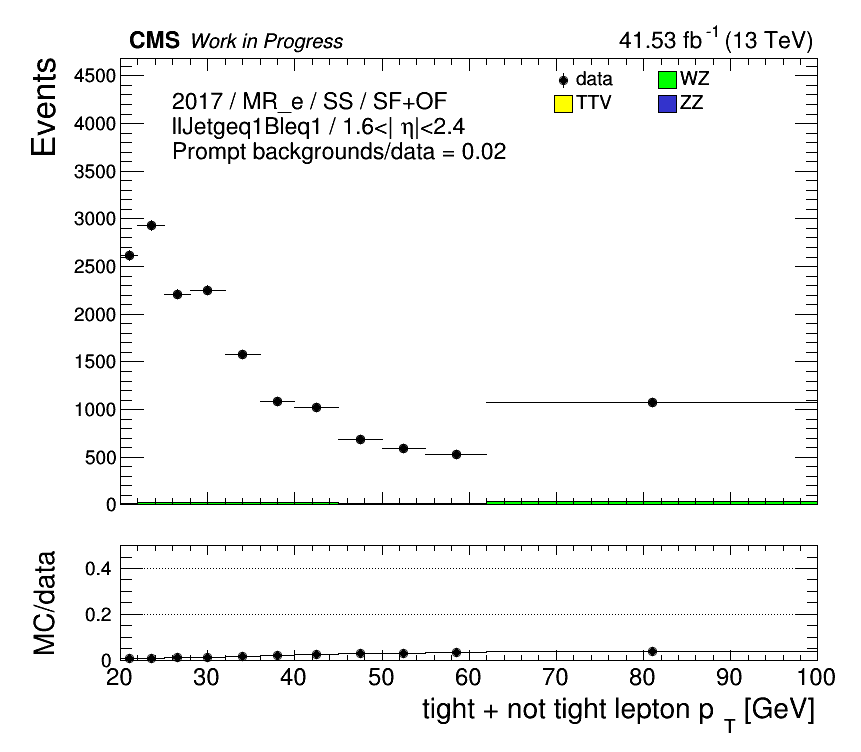
\includegraphics[width=0.45\textwidth]{figures/Part3/Nonprompt/MR/FlepPt}&
 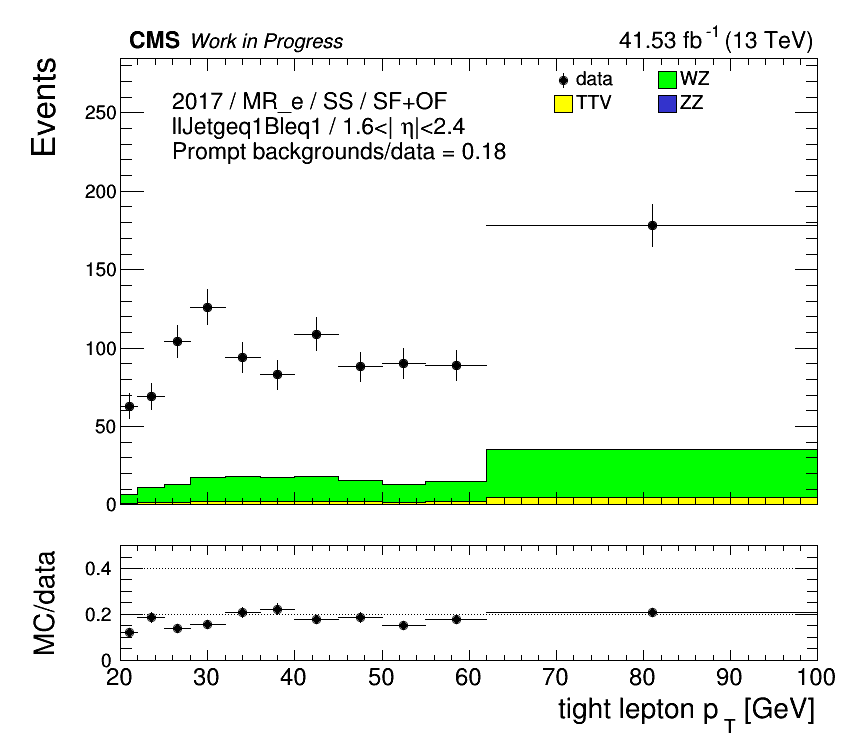
\includegraphics[width=0.45\textwidth]{figures/Part3/Nonprompt/MR/TlepPt} \\
 \end{tabular}
 \caption{Distribution of lepton $p_{T}$ in an electron \emph{fake} efficiency MR (2017). In this particular example: both $e+e$ (Same-Sign-Same-Flavor) and $e+\mu$ (Same-Sign-Opposite-Flavor) pair are considered. At least one jet and at most one b-tag jet are required (the second jet multiplicity bin). \emph{Probe} electron is required to have $1.6<|\eta|<2.4$ (the third $\eta$ bin). Contamination from prompt backgrounds are estimated with MC simulation. From left to right: \emph{tight+not tight} electron, only \emph{tight} electron.}
 \label{fig:MRexample}
 \end{center}
\end{figure}

\begin{figure}[tbh!]
 \begin{center}
 \begin{tabular}{c}
 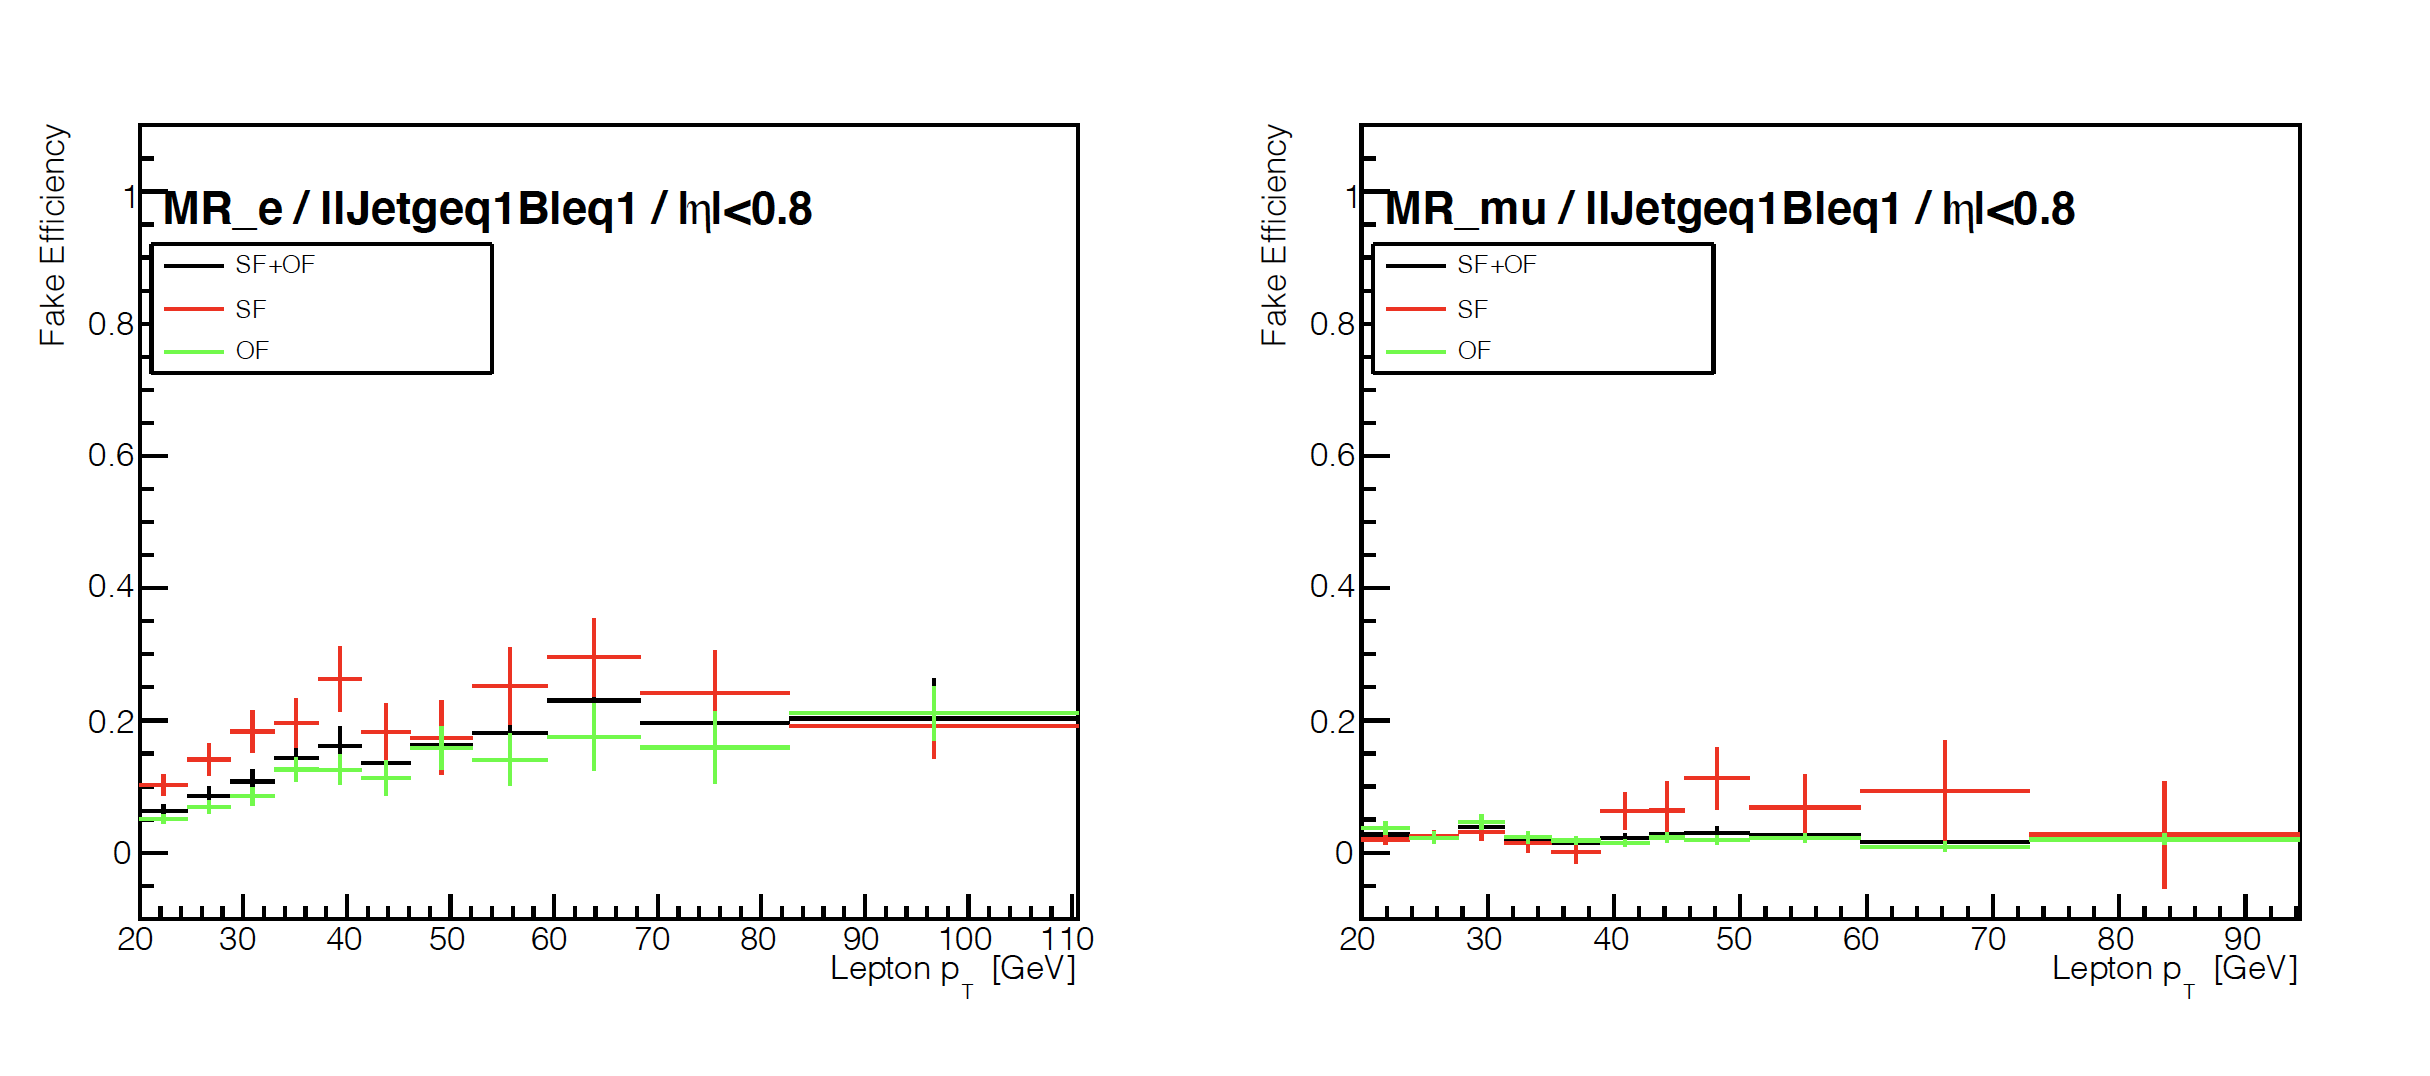
\includegraphics[width=0.85\textwidth]{figures/Part3/Nonprompt/MR/fake_eff}
 \end{tabular}
 \caption{Fake efficiency measured in 2017 data. These plots correspond to the first $|\eta|$ bin ($|\eta|<$0.8) and the second jet multiplicity bin. Error bars displayed in these plots include statistical uncertainty only. From left to right: electron $f$, muon $f$.}
 \label{fig:fake_eff}
 \end{center}
\end{figure}

The dependency of $f$ on background composition is also reflected in the difference between $f$ measured with different flavor compositions. For electrons, the \emph{fake} efficiency measured with $e+\mu$ selection is visibly different than the \emph{fake} efficiency measured with $e+e$ selection, which could suggest:

\begin{itemize}
\item \emph{Fake} electrons that originate from the decays of b-quarks have a lower probability of being selected by \emph{tight} selection than \emph{fake} electrons coming from Z+jets events.
\item The Same-Sign $e+e$ selection is contaminated with \emph{real} electrons and, to a less extent, the Same-Sign $e+\mu$ selection.
\end{itemize}

Events that have two same-sign electrons with an invariant mass between 76 GeV and 106 GeV are removed from MR to suppress the charge-flip effect of electrons. No such cut has been introduced to muon MR due to the negligible rate of charge-flip in muons.

Lepton selections listed in Table \ref{tab:looseandtight} are referred to as \emph{baseline}, which has been optimized to provide a robust non-prompt estimate. Variation of the \emph{basline} selection has also been studied. 

There is a trade-off between muon $r$ and $f$ when changing the isolation requirement (See Figure \ref{fig:f_muoniso}-\ref{fig:r_muoniso}). While it is ideal to reduce statistical uncertainties by loosening the \emph{loose} definition, a low \emph{real} efficiency should also be avoided. This change proves to have a minor effect on the overall estimate.
 
\begin{figure}[tbh!]
 \begin{center}
 \begin{tabular}{ccc}
 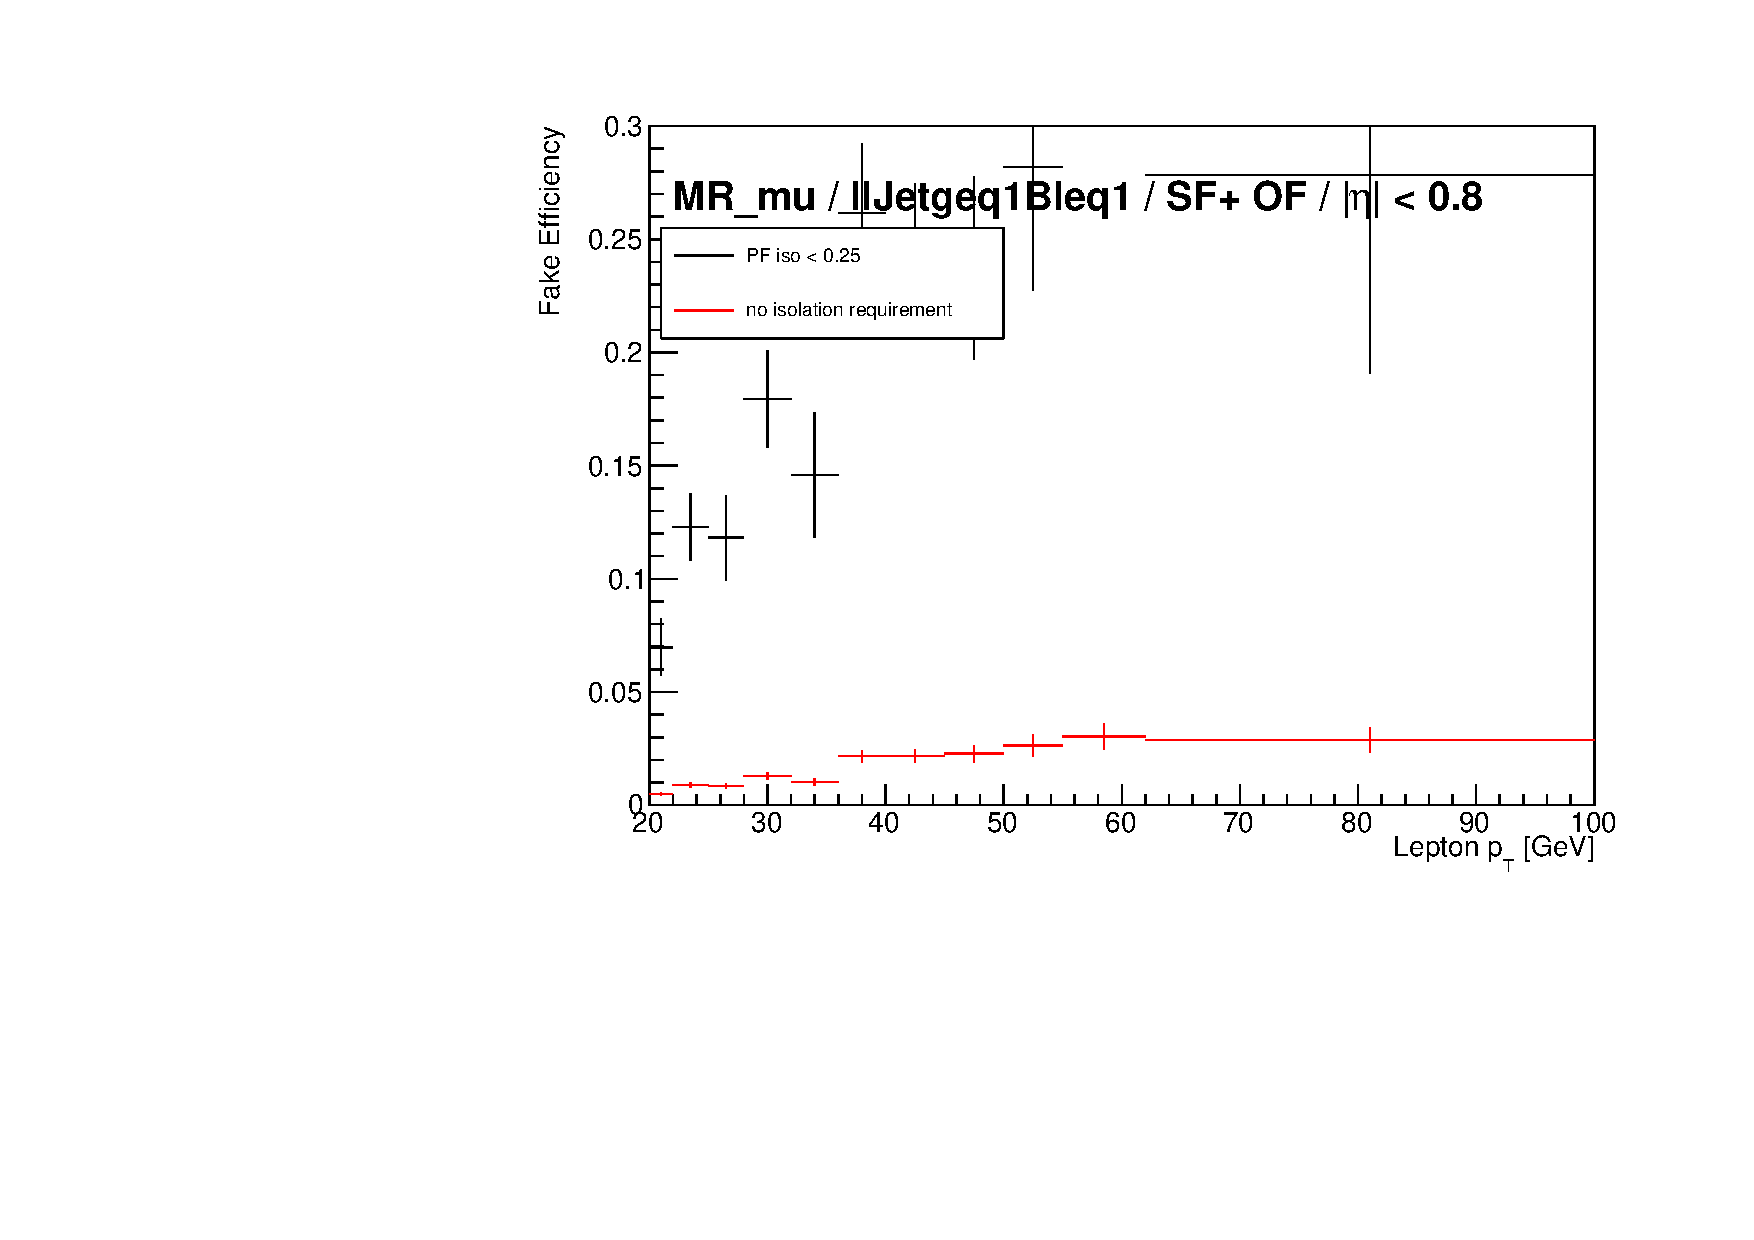
\includegraphics[width=0.32\textwidth]{figures/Part3/Nonprompt/MR/f_muoniso_barrel}&
 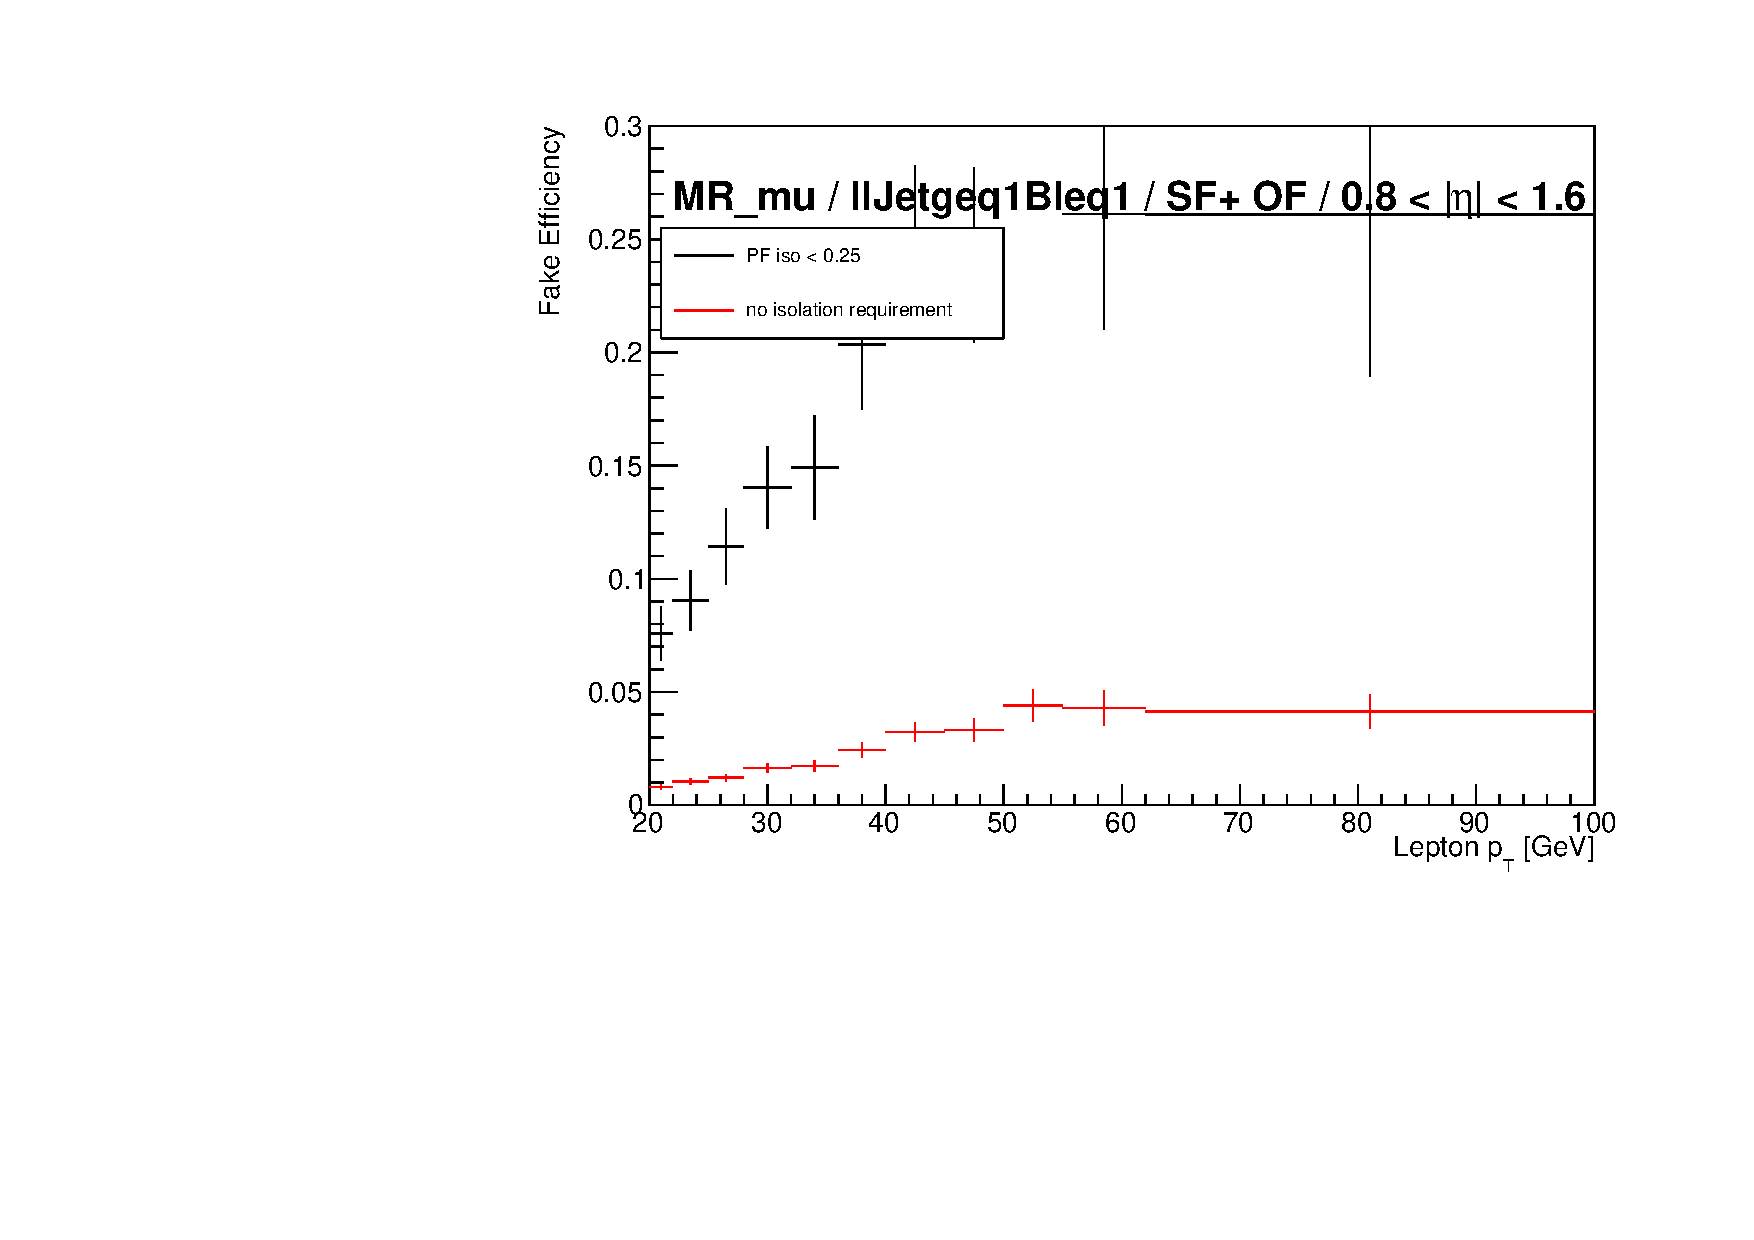
\includegraphics[width=0.32\textwidth]{figures/Part3/Nonprompt/MR/f_muoniso_transition}&
 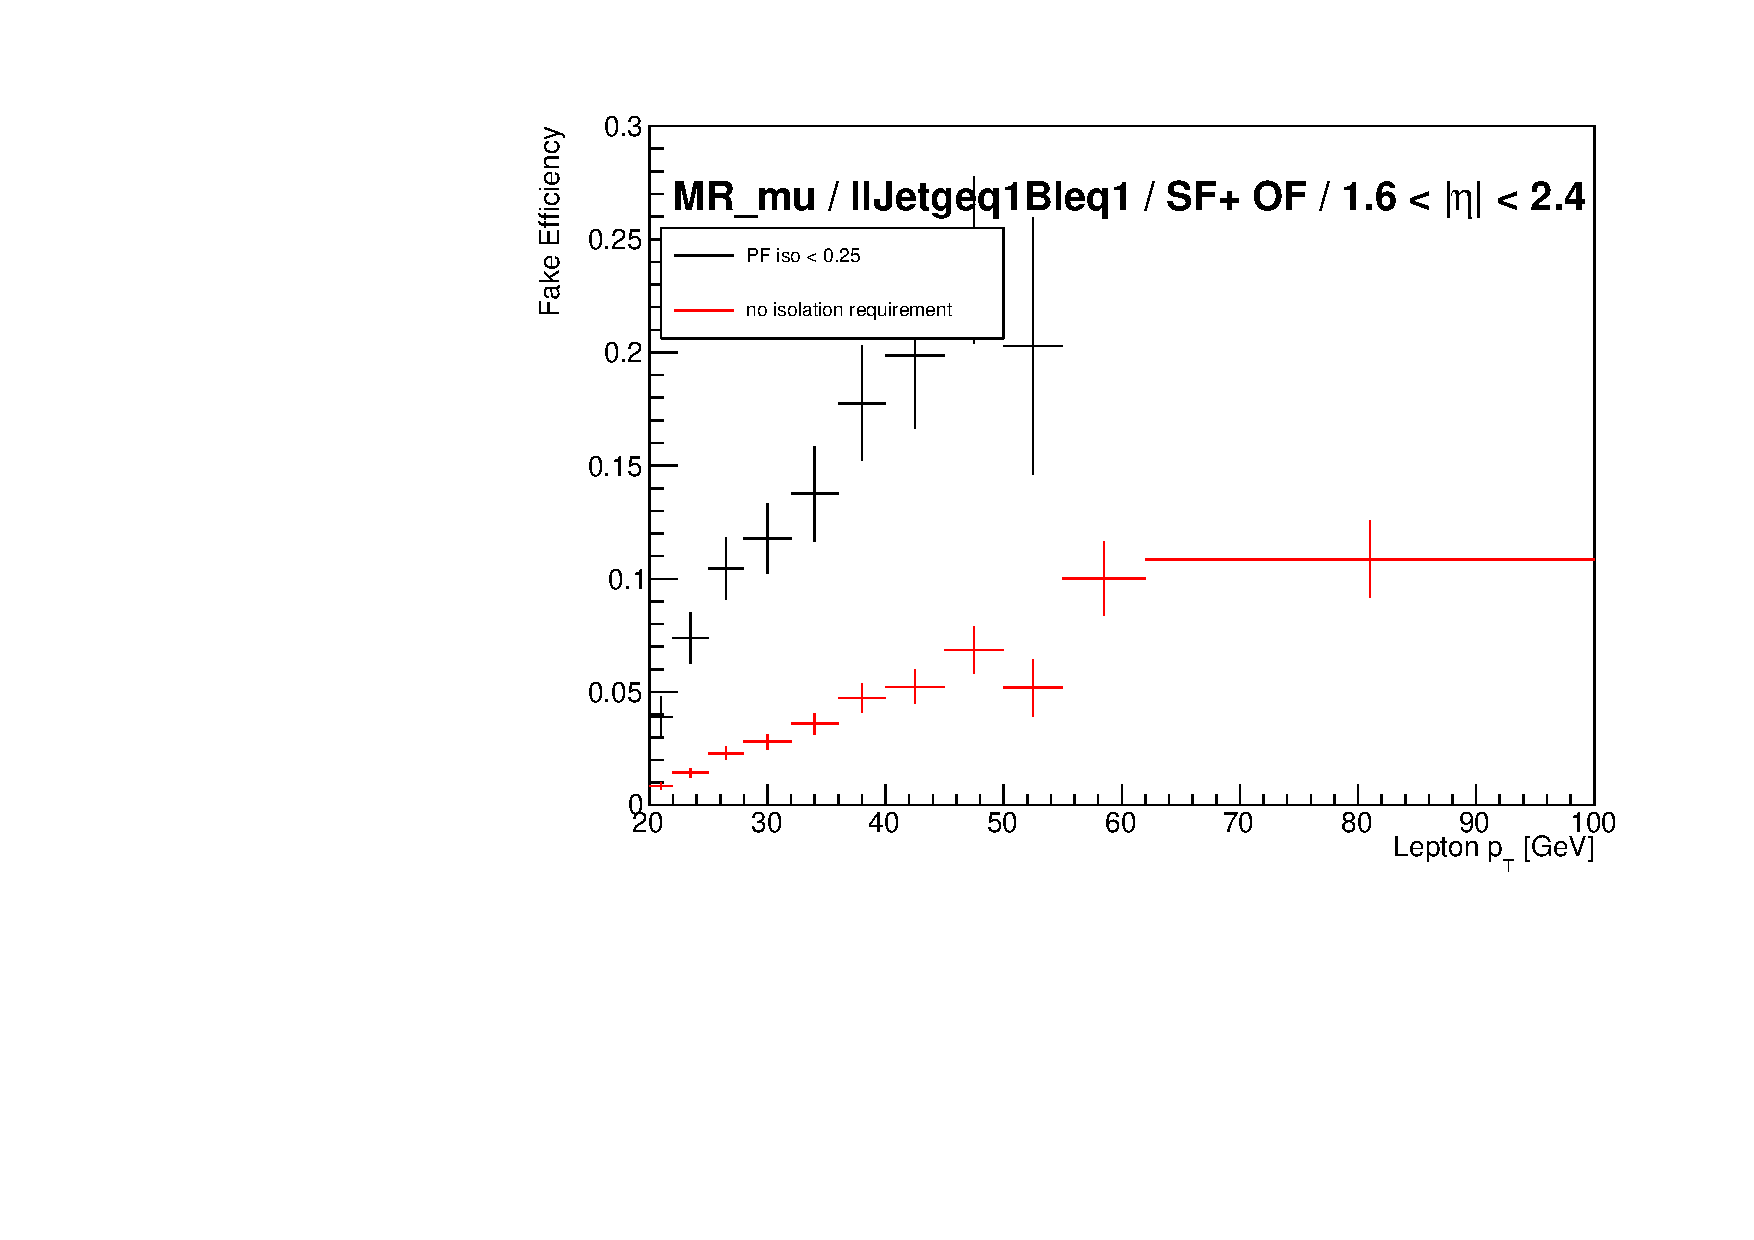
\includegraphics[width=0.32\textwidth]{figures/Part3/Nonprompt/MR/f_muoniso_endcap} \\
 \end{tabular}
 \caption{Comparison of the muon \emph{fake} efficiencies measured with isolation requirement in \emph{loose} definition (2017 datasets). From left to right: $|\eta|<$0.8, 0.8$<|\eta|<$1.6, 1.6$<|\eta|<$2.4.}
 \label{fig:f_muoniso}
 \end{center}
\end{figure}

\begin{figure}[tbh!]
 \begin{center}
 \begin{tabular}{ccc}
 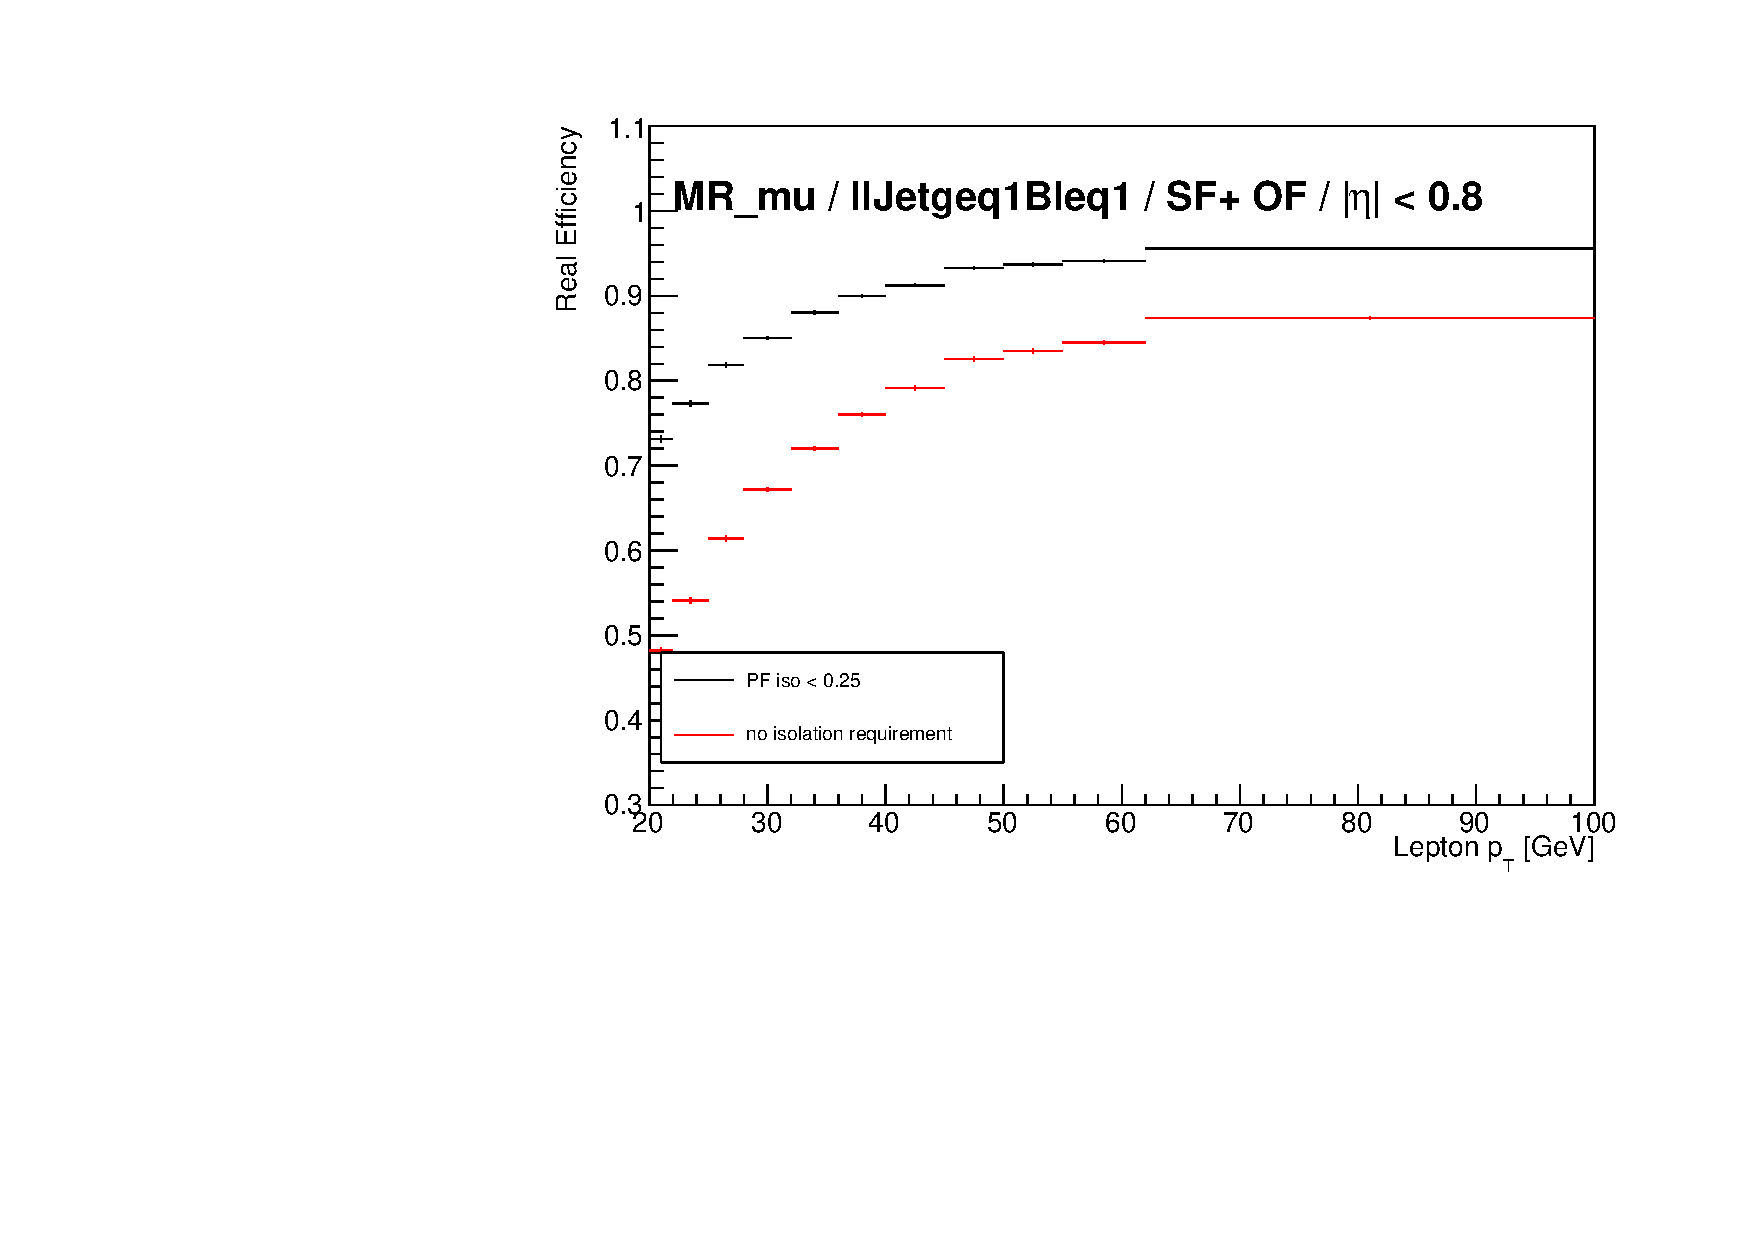
\includegraphics[width=0.32\textwidth]{figures/Part3/Nonprompt/MR/r_muoniso_barrel}&
 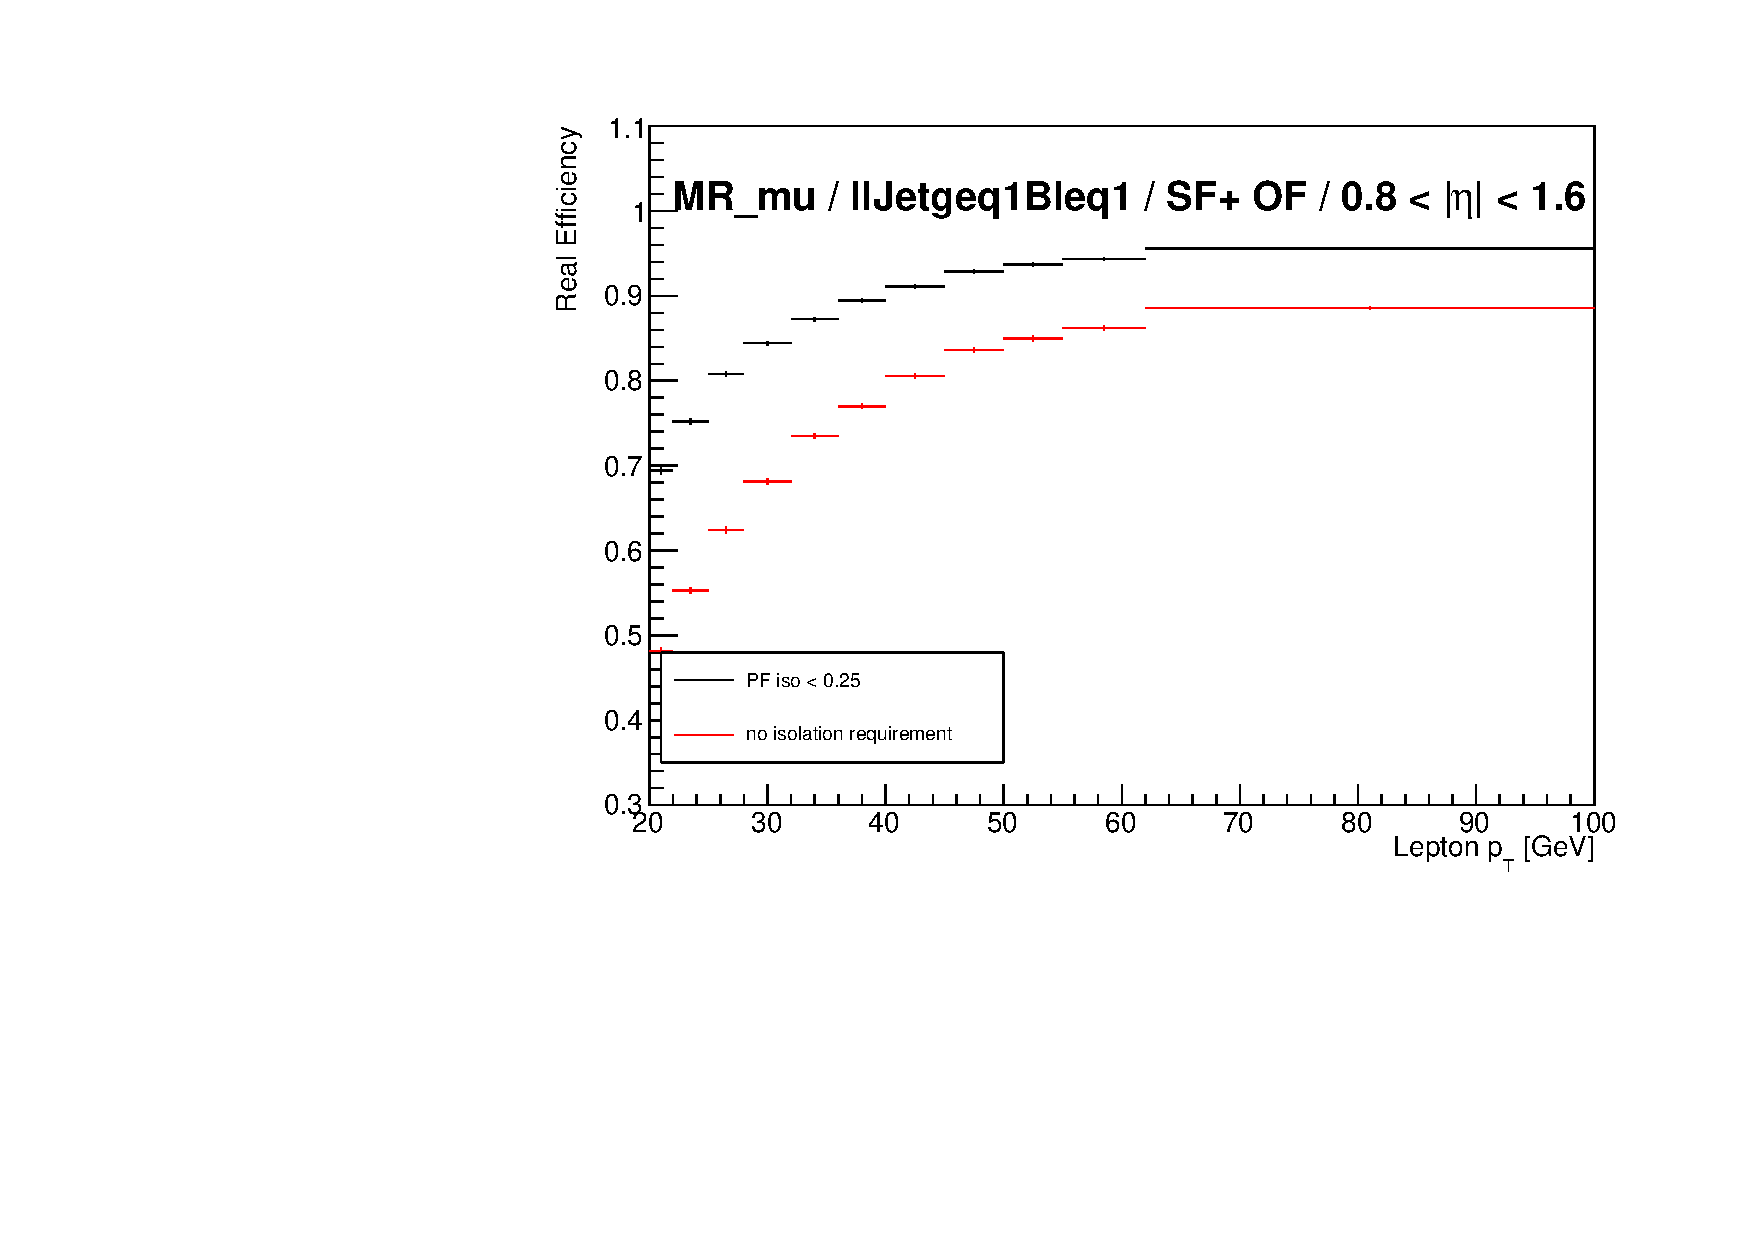
\includegraphics[width=0.32\textwidth]{figures/Part3/Nonprompt/MR/r_muoniso_transition}&
 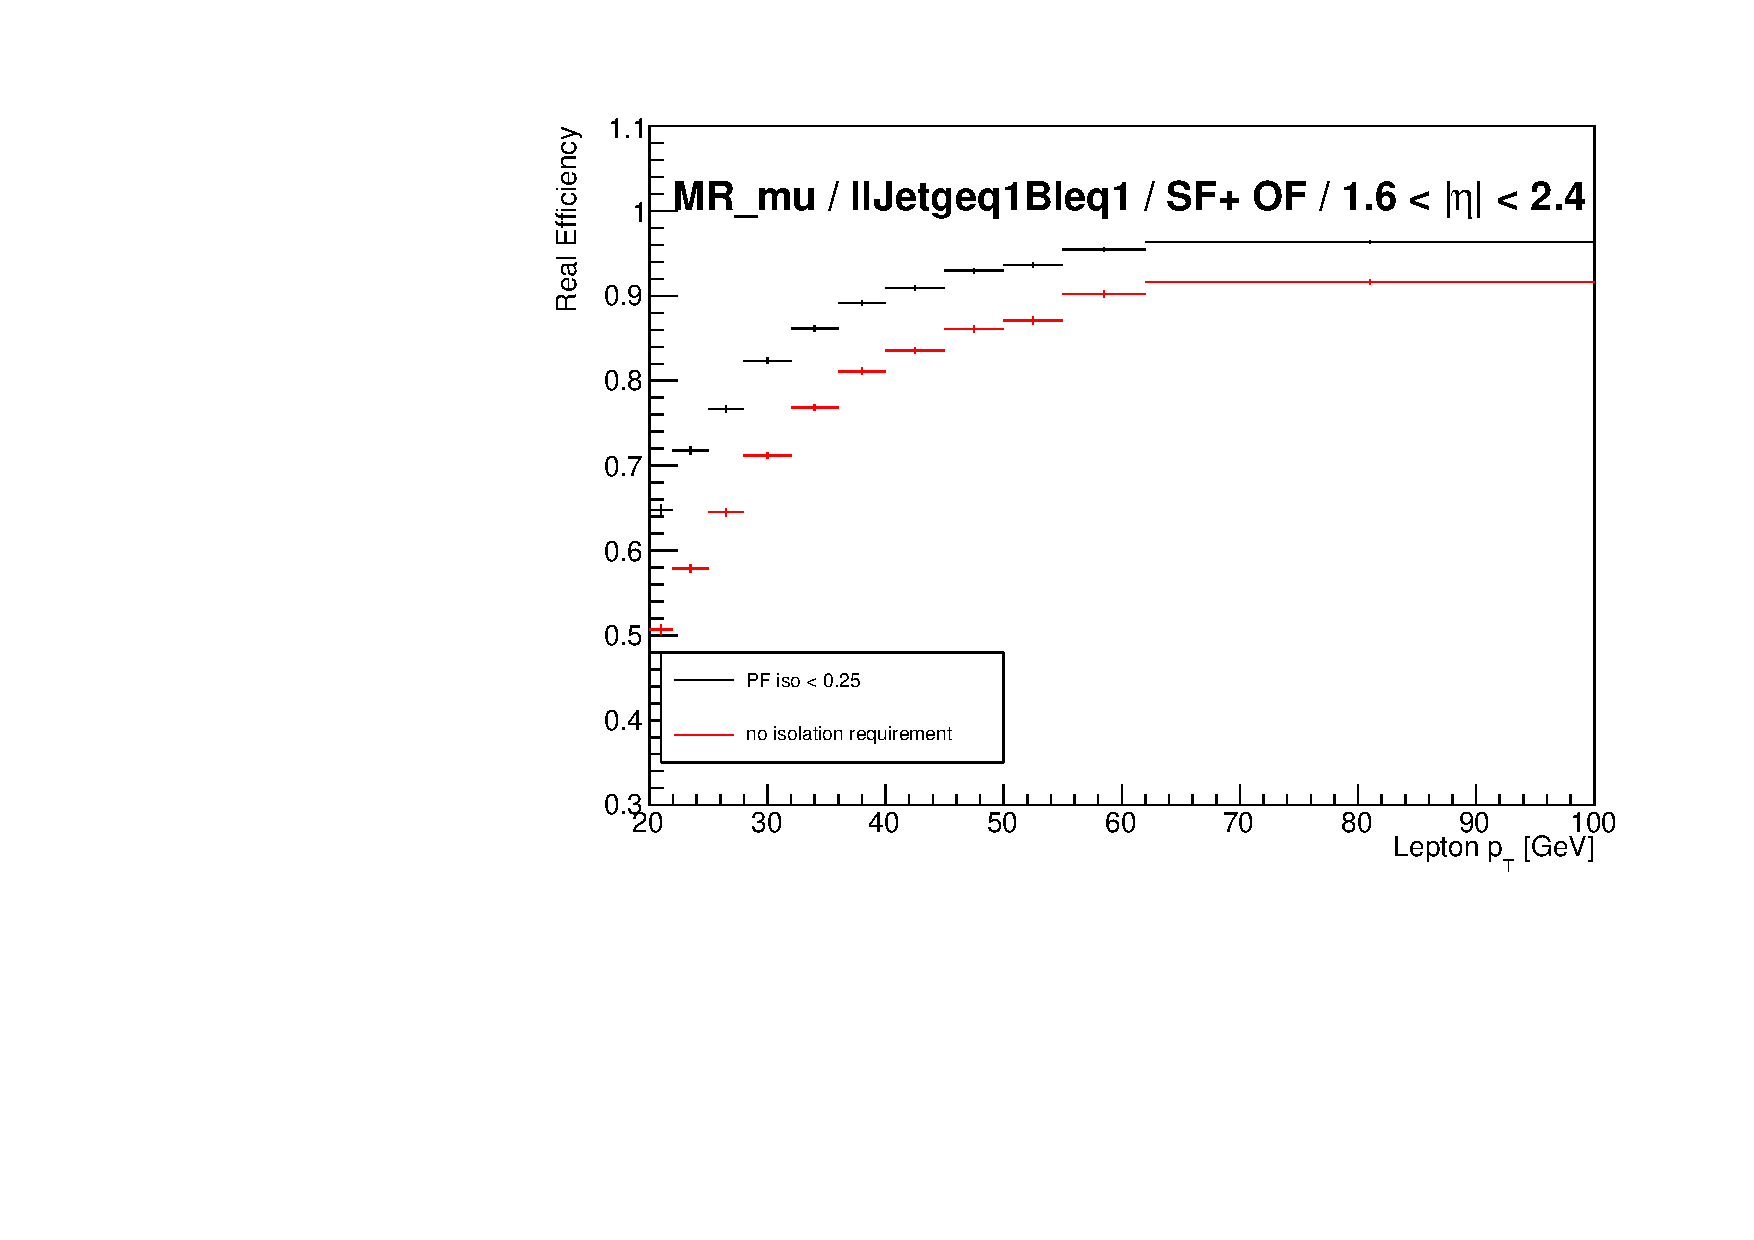
\includegraphics[width=0.32\textwidth]{figures/Part3/Nonprompt/MR/r_muoniso_endcap} \\
 \end{tabular}
 \caption{Comparison of the muon \emph{real} efficiencies measured with different \emph{loose} definition (2017 datasets). From left to right: $|\eta|<$0.8, 0.8$<|\eta|<$1.6, 1.6$<|\eta|<$2.4.}
 \label{fig:r_muoniso}
 \end{center}
\end{figure}

\begin{figure}[tbh!]
 \begin{center}
 \begin{tabular}{c}
 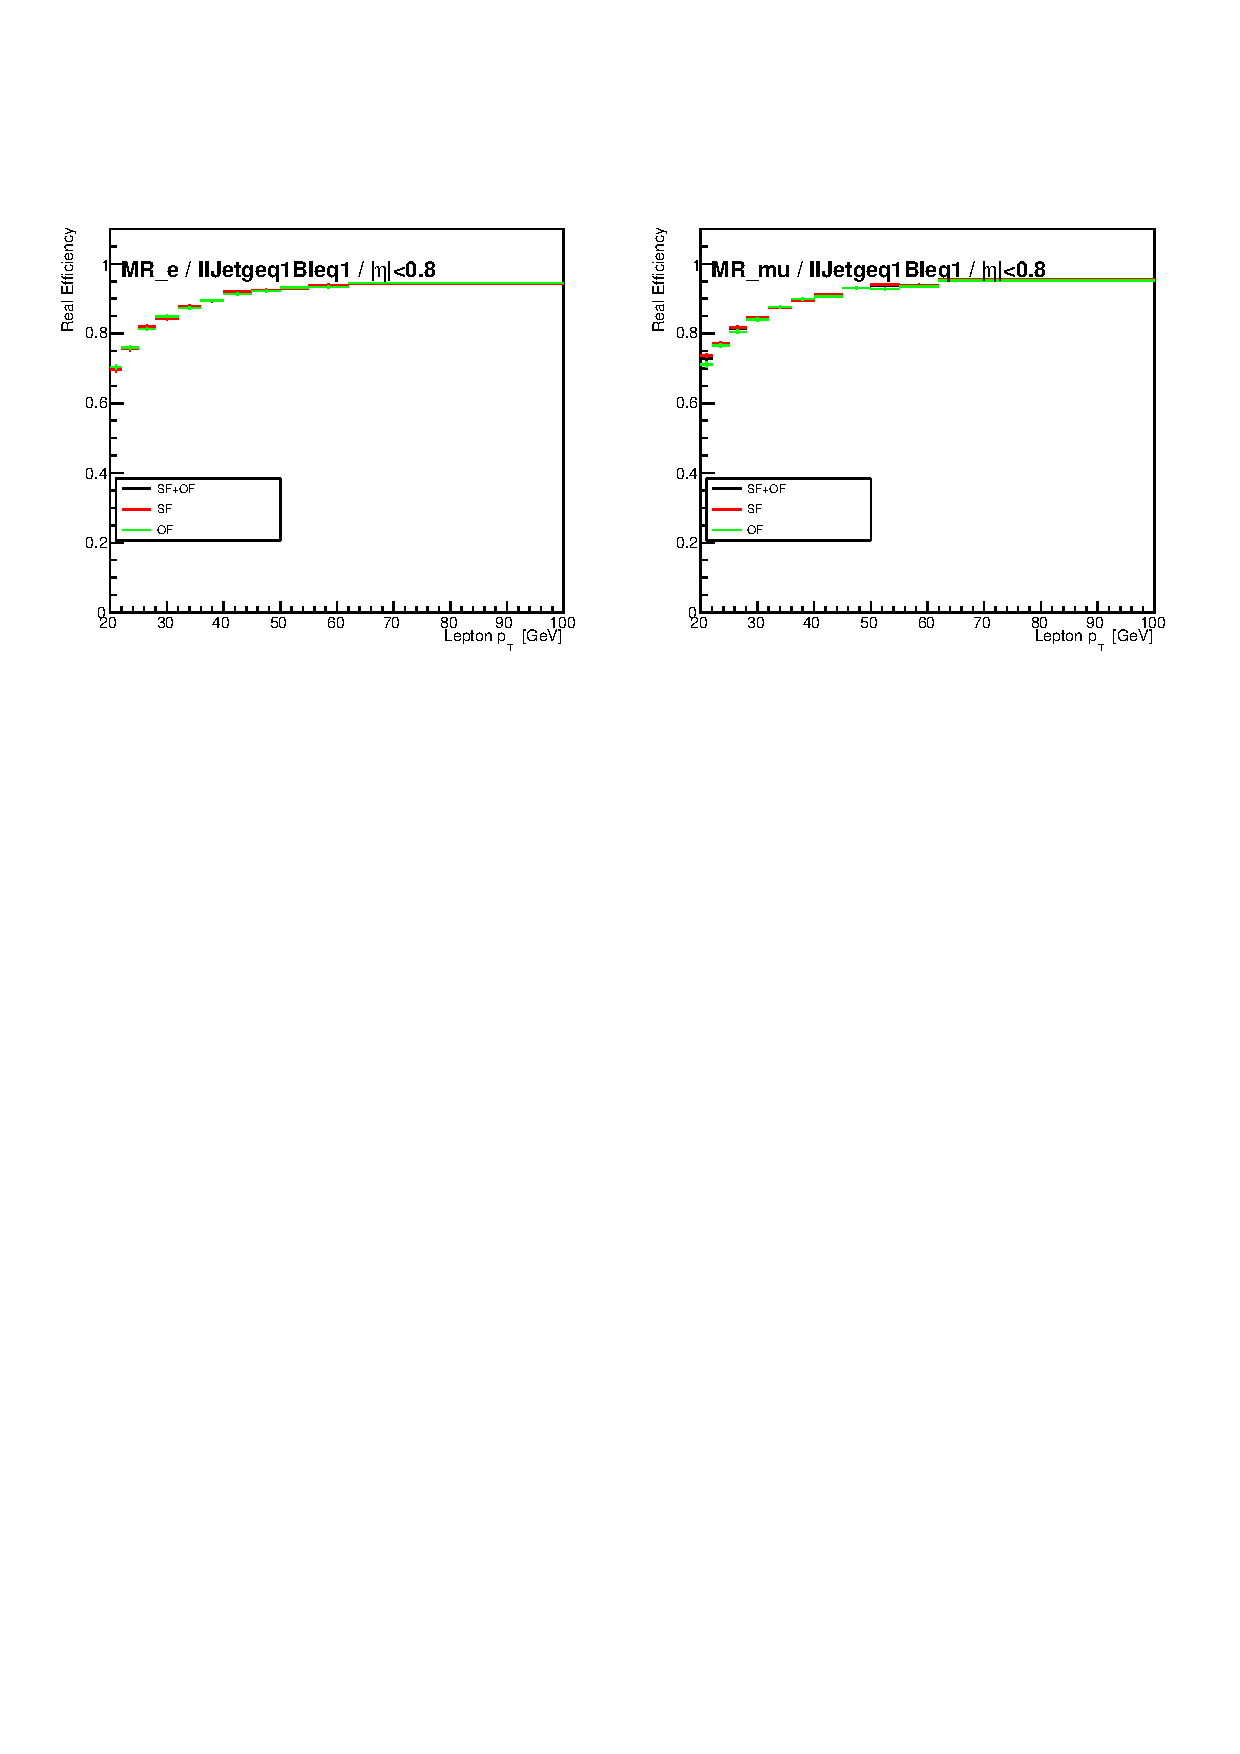
\includegraphics[width=0.85\textwidth]{figures/Part3/Nonprompt/MR/real_eff}
 \end{tabular}
 \caption{\emph{Real} efficiency measured in simulated $t\bar{t}$ events (2017). These plots correspond to the first $|\eta|$ bin ($|\eta|<$0.8) and the second jet multiplicity bin. Error bars displayed in these plots include statistical uncertainty only. From left to right: electron $r$, muon $r$.}
 \label{fig:real_eff}
 \end{center}
\end{figure}

The \emph{real} efficiency $r$ is estimated with simulated $t\bar{t}$ events in an Opposite-Sign dilepton region. The same lepton selection (See Table \ref{tab:looseandtight}) is used to perform Tag-and-Probe. The leading lepton in $p_{T}$ is used as a \emph{tag} while the sub-leading lepton (with opposite sign) is taken as a \emph{probe}. The variation of $r$ between $e+e$ and $e+\mu$ flavor combination is negligible (See Figure \ref{fig:real_eff}). Therefore, only $e+\mu$ events are used to measure \emph{real} efficiency in order to minimize the contamination of \emph{fake} leptons.

The selection criteria for $r/f$ measurement region is summarized in Table \ref{tab:MR}. The latest version of the \emph{real} and \emph{fake} efficiency is summarized in autoref{sec:RandF}.

\begin{table}[th]
\sffamily
\centering
\resizebox{\textwidth}{!}{ 
\begin{tabular}{cccccccc}
\hline 
Observable                 &jet bin          & $\#$ of selected leptons & lepton flavor composite  & $|\Sigma_iC_i|$ & OffZ               &  njet$>=$1  &nbjet$<=$1\\ \hline \hline
\multirow{2}{*}{$f$}     & 0 jet                & 2                                & any                                   & 1                       & \checkmark     & -                    & -   \\  
                                   & 1 or more jet  & 2                                &  any                                  & 1                         & \checkmark     & \checkmark & \checkmark\\ \hline
\multirow{2}{*}{$r$}    & 0 jet                & 2                                 & $e\mu$ only                     & 0                        & \checkmark     & -                      & -     \\  
                                 & 1 or more jet  & 2                                  & $e\mu$ only                      & 0                        & \checkmark      & \checkmark & \checkmark \\ \hline   
\end{tabular}
}
\caption{Summary of the cuts applied to the $r$/$f$ measurement region.}
\label{tab:MR}
\end{table}
%%%%%%%%%%%%%%%%%%%%%%%%%%%%%%%%%%%%%%%%%%%%%%%%%%%%%%%%%%%%%
%%%%%%%%%%%%%%%%%%%%%%%%%%%%%%%%%%%%%%%%%%%%%%%%%%%%%%%%%%%%%
\section{Validation of the Matrix Method}
\label{sec:MMVR}

The performance of the matrix method is validated using three regions that are tangential to the SR, referred to as VRs. In these VRs, prompt backgrounds are estimated with MC simulation while non-prompt backgrounds are estimated with the matrix method. A summary of the selections applied to these VRs is given in autoref{sec:selection}.4. 

Distribution of lepton lepton $\eta$ and jet multiplicity are shown in Figure \ref{fig:VR_matrix_eee}-\ref{fig:VR_matrix_mumumu}. Distributions of other variables are included in autoref{sec:VRmatrix}

\begin{figure}[tbh!]
 \begin{center}
 \begin{tabular}{cc}
 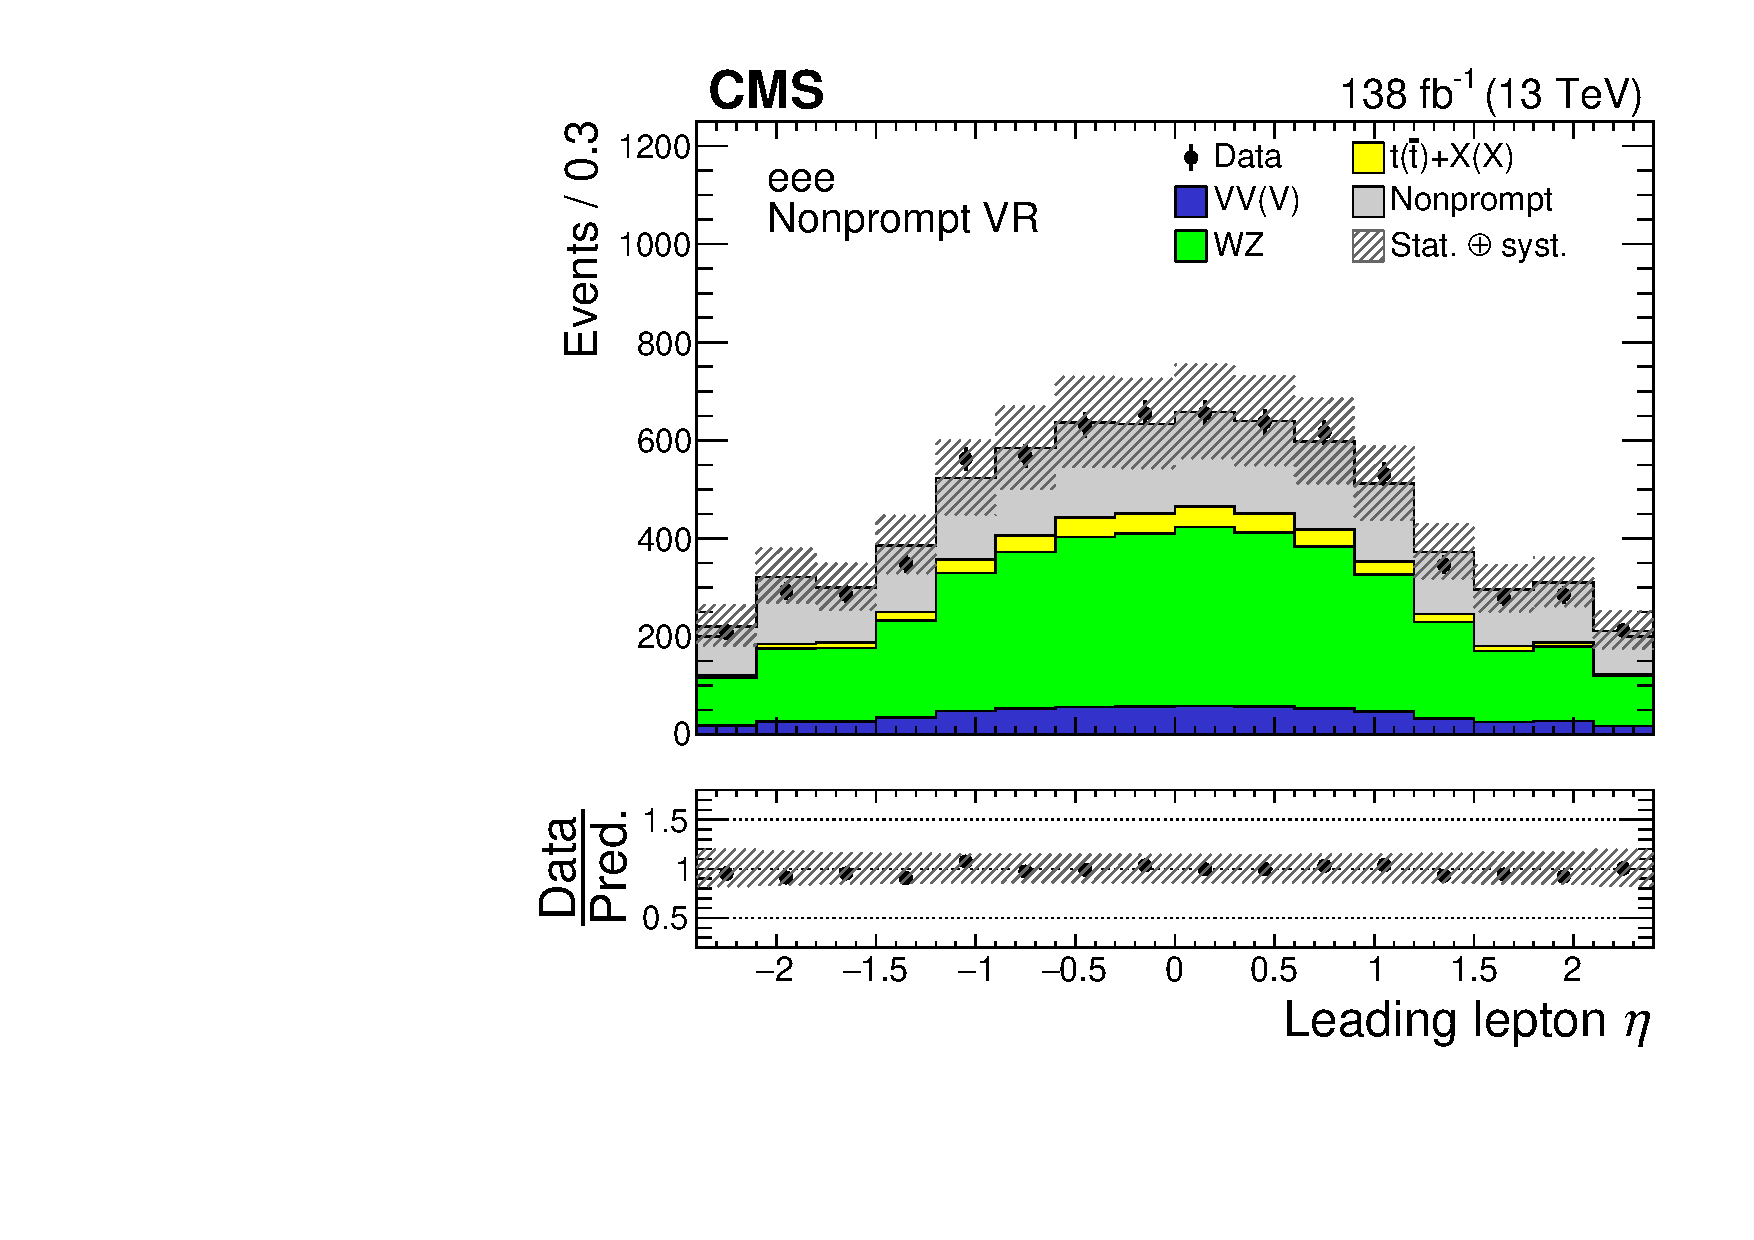
\includegraphics[width=0.45\textwidth]{figures/Part3/Nonprompt/VR/eee/lep1Eta}&
 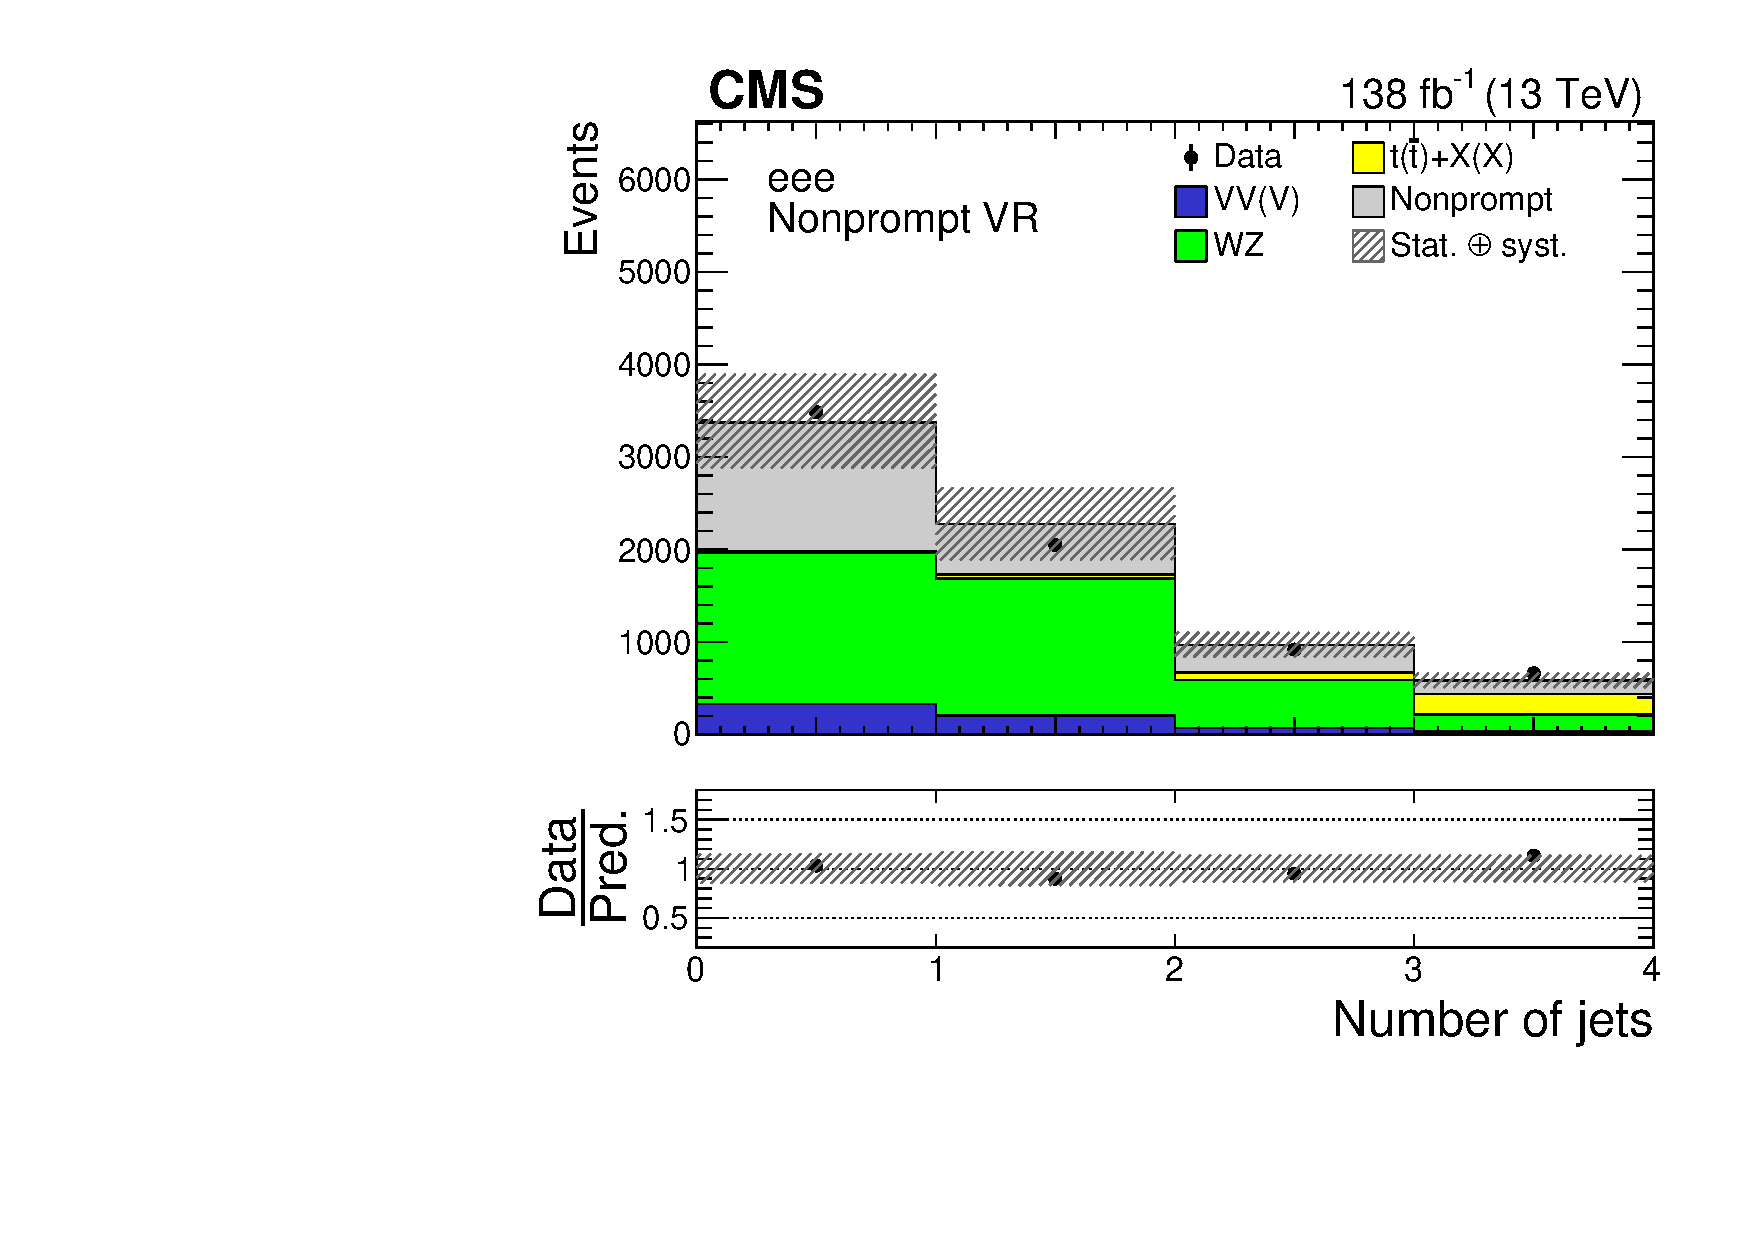
\includegraphics[width=0.45\textwidth]{figures/Part3/Nonprompt/VR/eee/njet} \\
 \end{tabular}
 \caption{Distributions of different kinematic variables estimated in VR with three electrons. From left to right: leading lepton $\eta$, jet multiplicity.}
 \label{fig:VR_matrix_eee}
 \end{center}
\end{figure}

\begin{figure}[tbh!]
 \begin{center}
 \begin{tabular}{cc}
  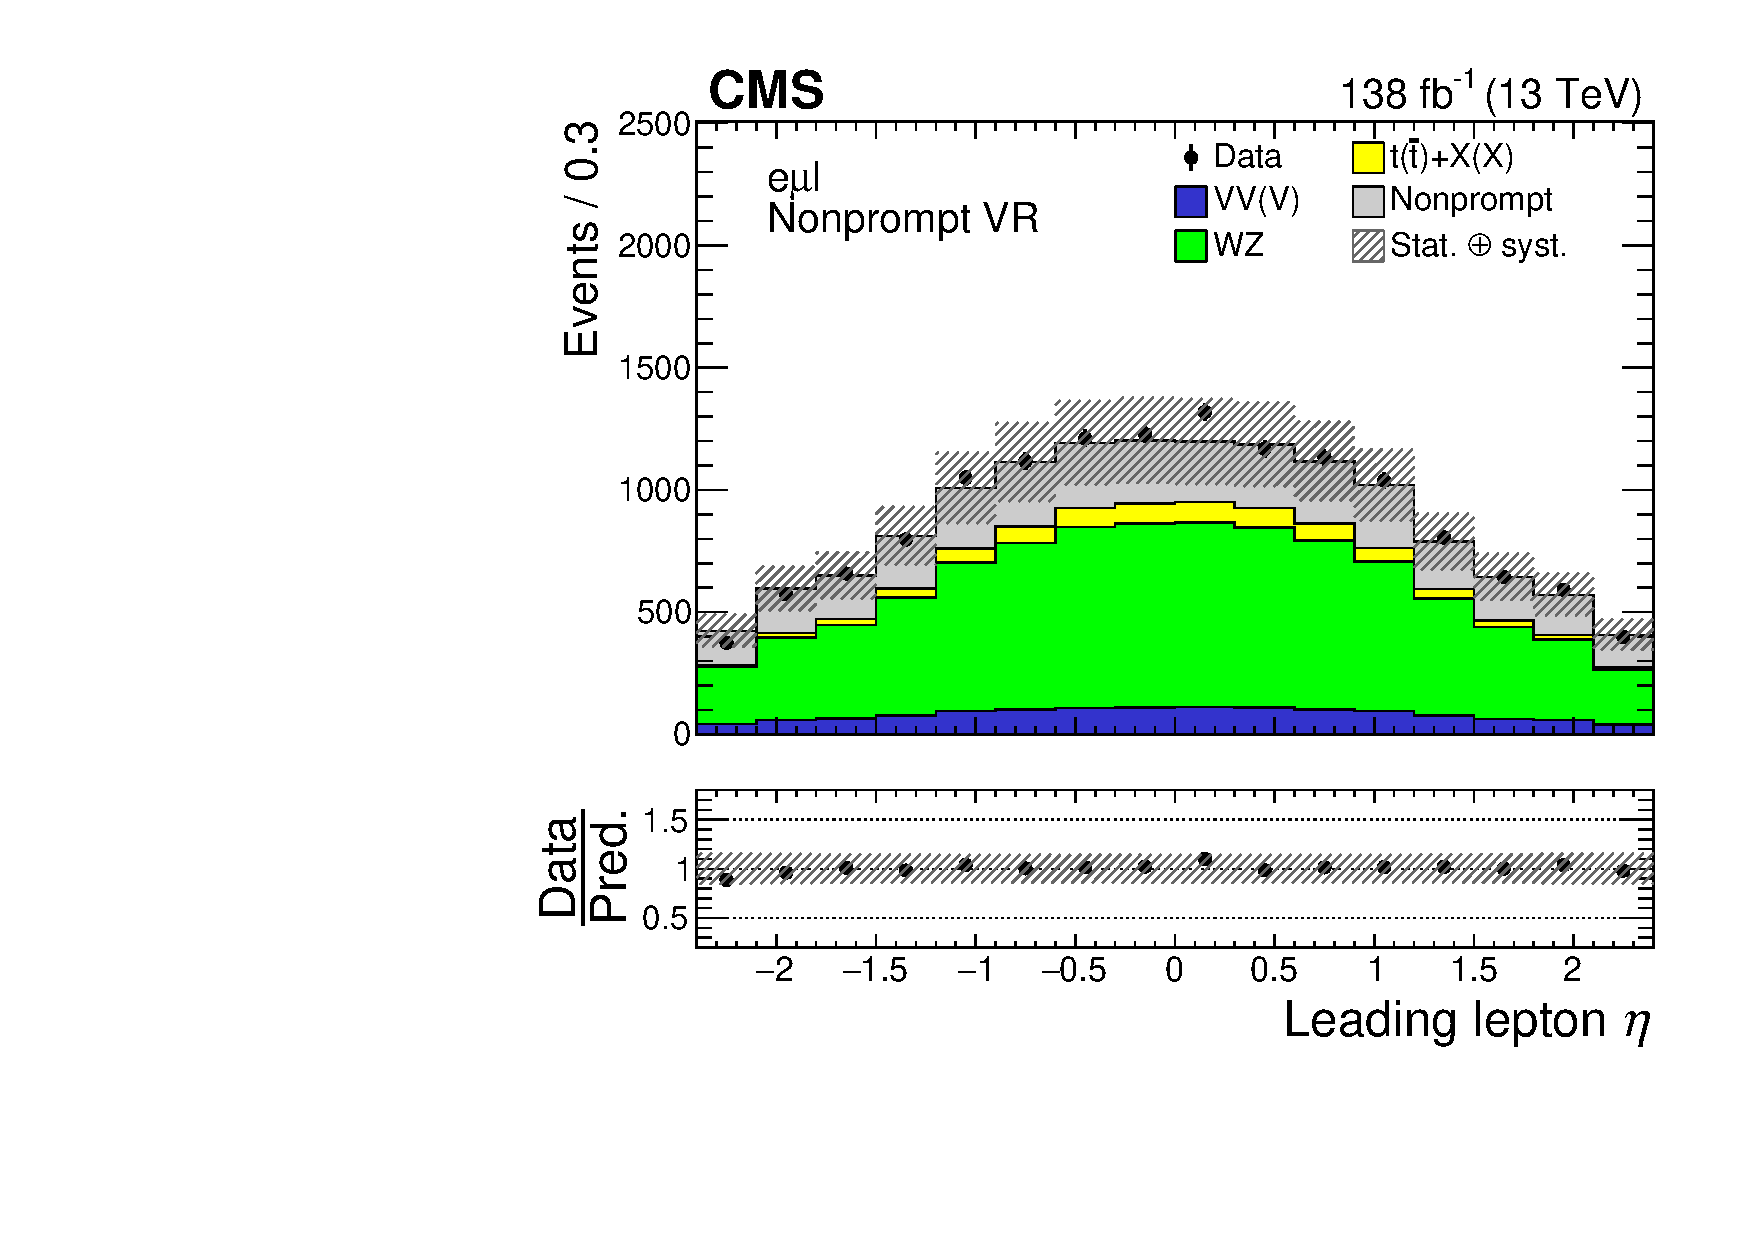
\includegraphics[width=0.45\textwidth]{figures/Part3/Nonprompt/VR/emul/lep1Eta}&
 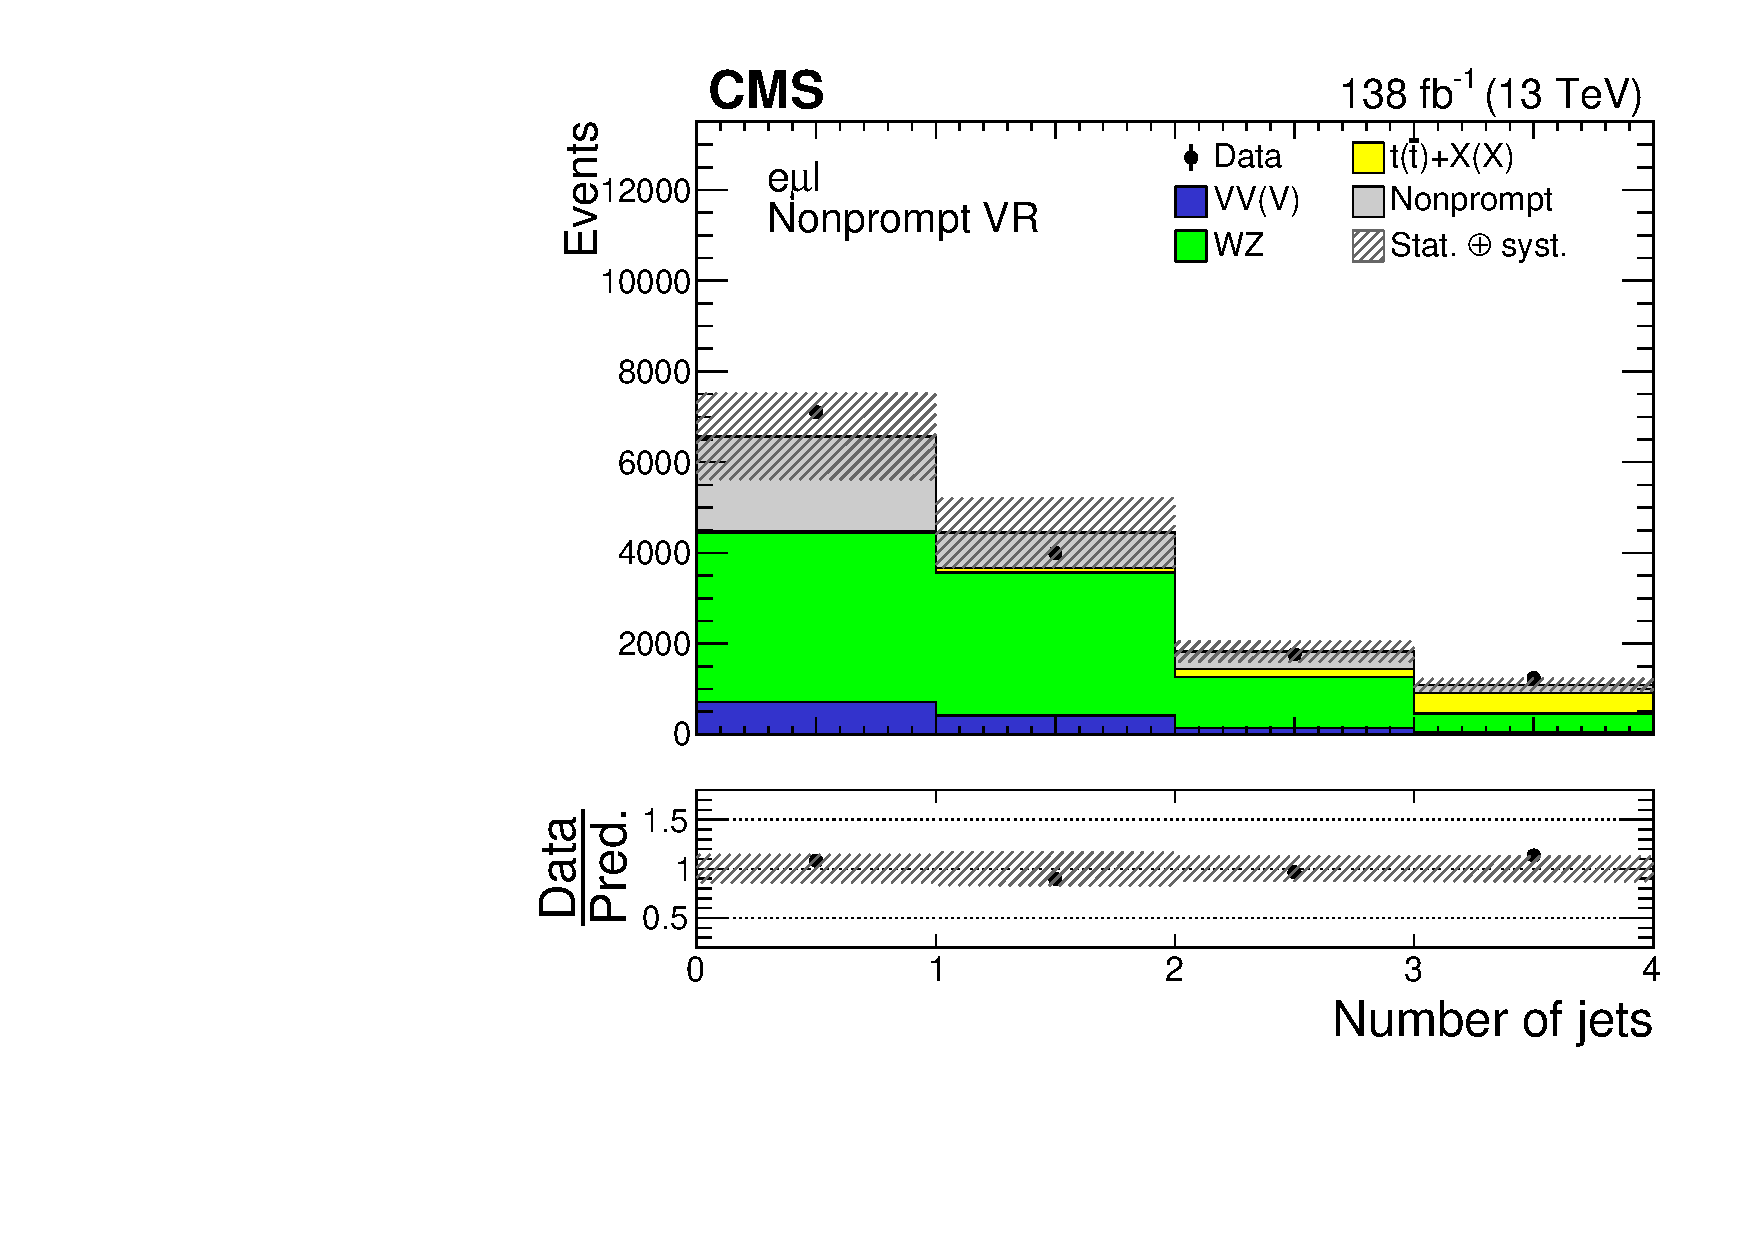
\includegraphics[width=0.45\textwidth]{figures/Part3/Nonprompt/VR/emul/njet} \\
 \end{tabular}
 \caption{Distributions of different kinematic variables estimated in VR with electron, muon and a third light lepton. From left to right: leading lepton $\eta$, jet multiplicity.}
 \label{fig:VR_matrix_emul}
 \end{center}
\end{figure}

\begin{figure}[tbh!]
 \begin{center}
 \begin{tabular}{cc}
   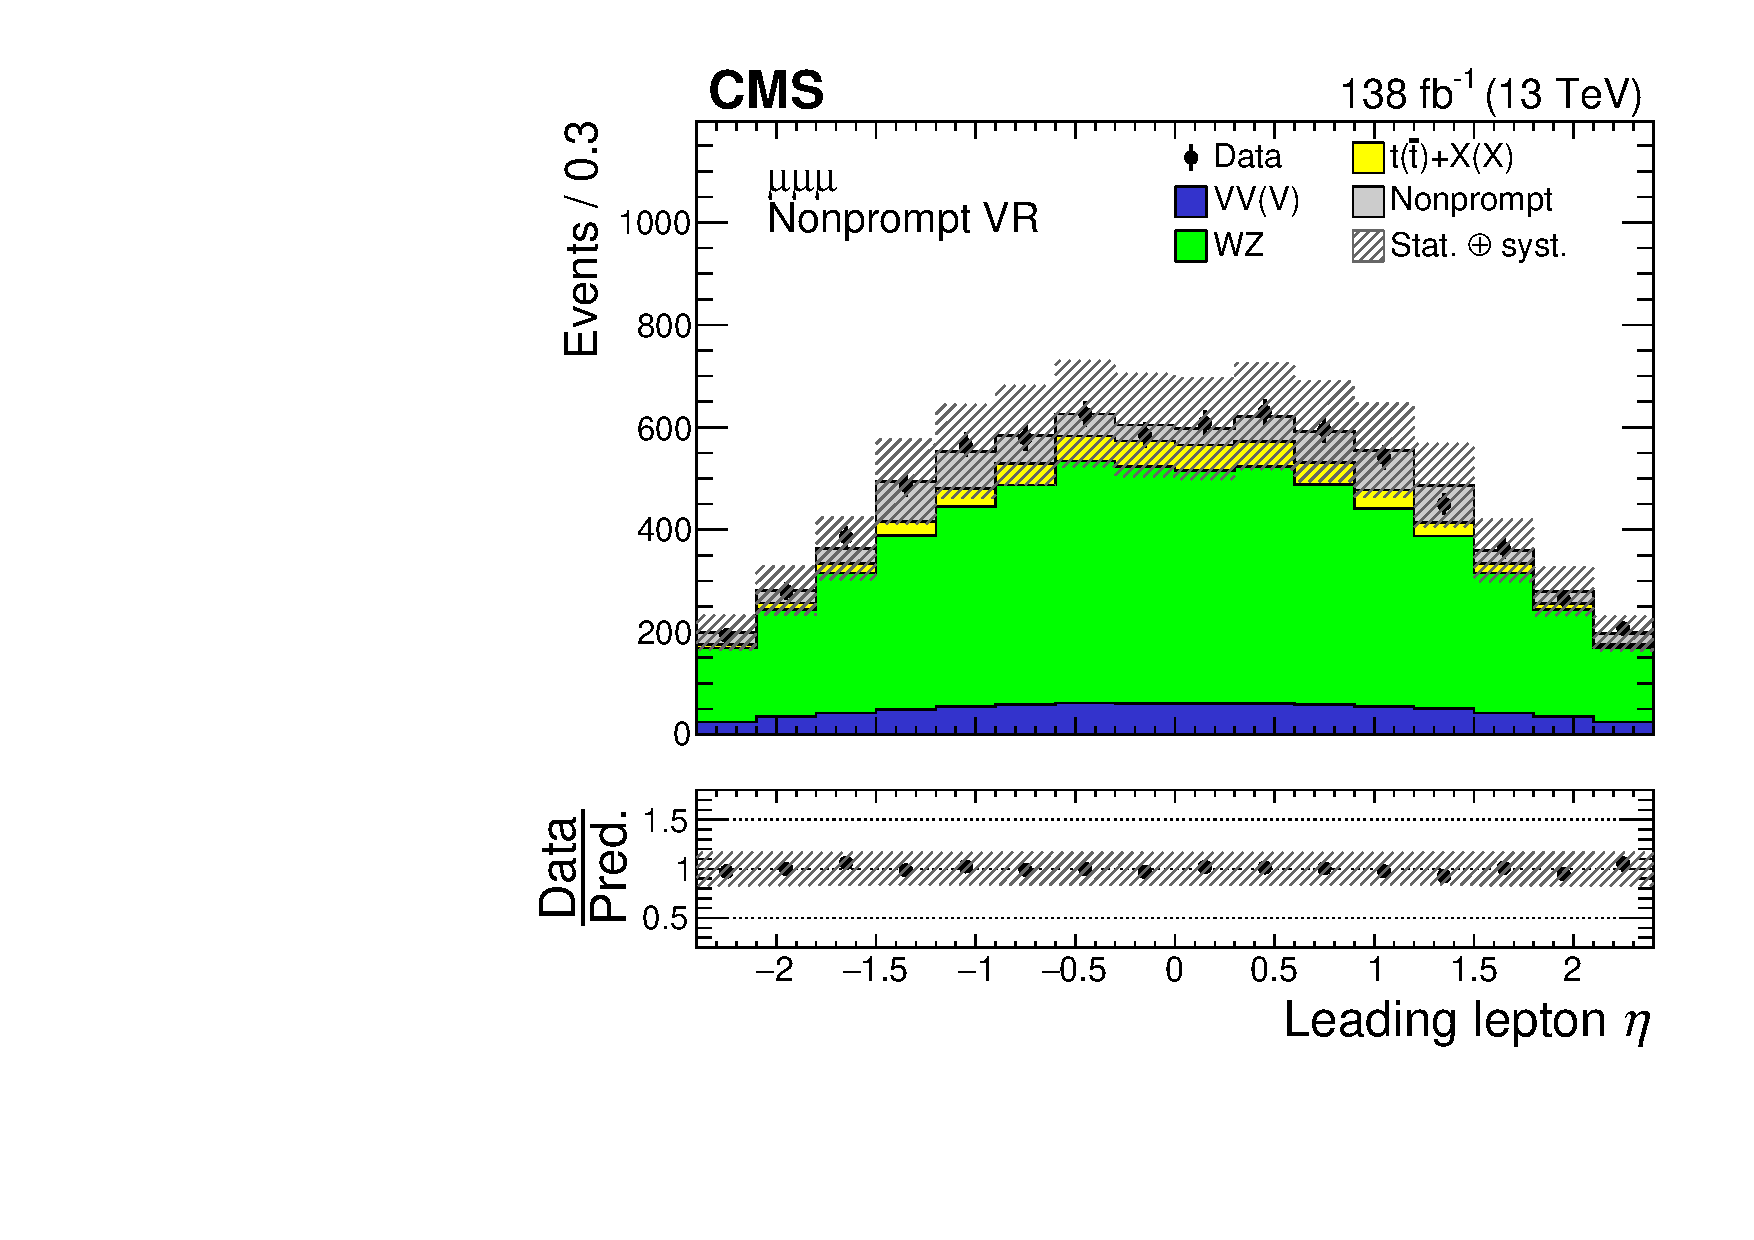
\includegraphics[width=0.45\textwidth]{figures/Part3/Nonprompt/VR/mumumu/lep1Eta}&
 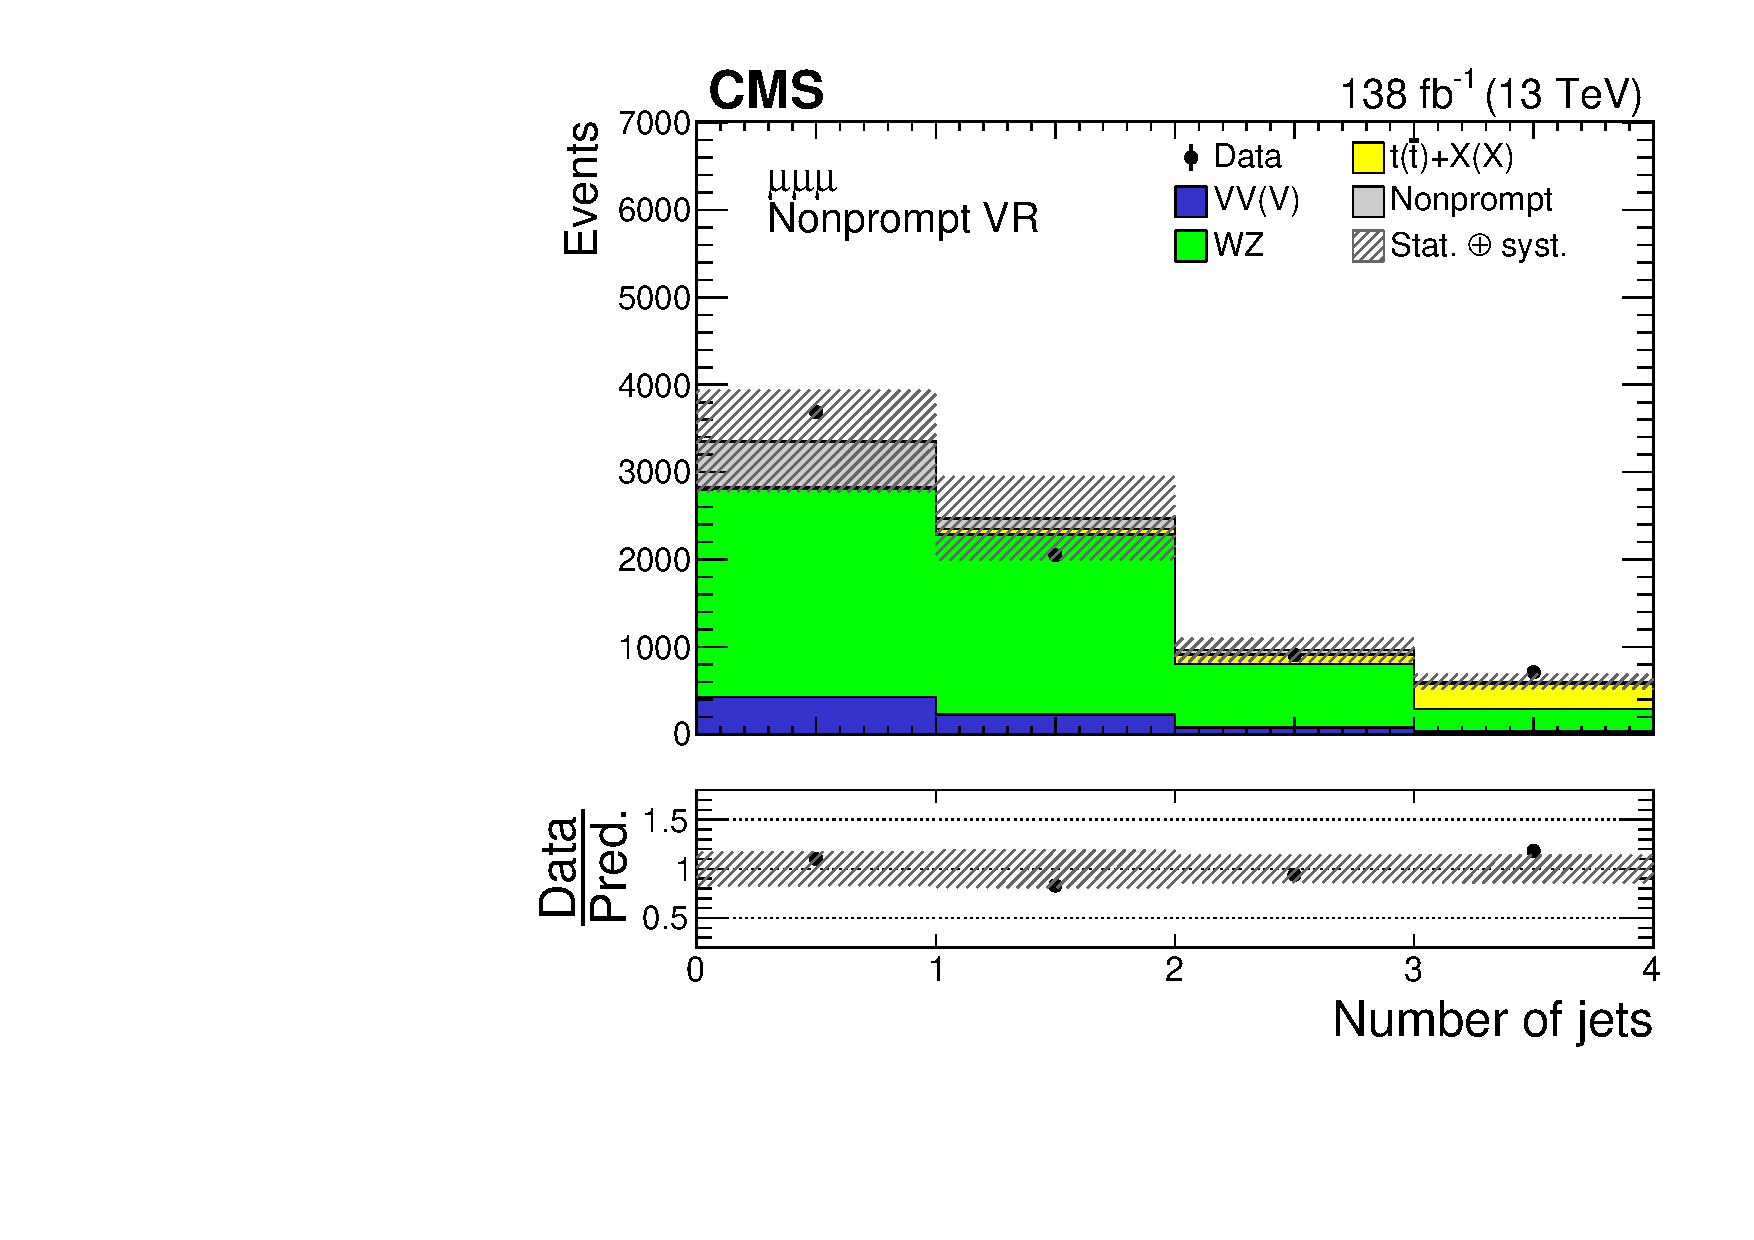
\includegraphics[width=0.45\textwidth]{figures/Part3/Nonprompt/VR/mumumu/njet} \\
 \end{tabular}
 \caption{Distributions of different kinematic variables estimated in VR with three muons. From left to right: leading lepton $\eta$, jet multiplicity.}
 \label{fig:VR_matrix_mumumu}
 \end{center}
\end{figure}
%%%%%%%%%%%%%%%%%%%%%%%%%%%%%%%%%%%%%%%%%%%%%%%%%%%%%%%%%%%%%
%%%%%%%%%%%%%%%%%%%%%%%%%%%%%%%%%%%%%%%%%%%%%%%%%%%%%%%%%%%%%
\section{Nonprompt estimate in SR}
\label{sec:MMSR}

The matrix method is used to estimate non-prompt backgrounds in the signal region due to its superior performance over other alternative methods (e.g. fake factor method discussed in autoref{sec:appendixnonprompt}). Distributions of leading lepton $\eta$, jet multiplicity, n-jet multiplicity, missing transverse energy, LFV-Top mass and Z mass are shown in Figure \ref{fig:SR_DataDriven_1}-\ref{fig:SR_DataDriven_2}. Distributions of other variables are included in autoref{sec:SRDataDriven}.

\begin{figure}[tbh!]
 \begin{center}
 \begin{tabular}{cc}
  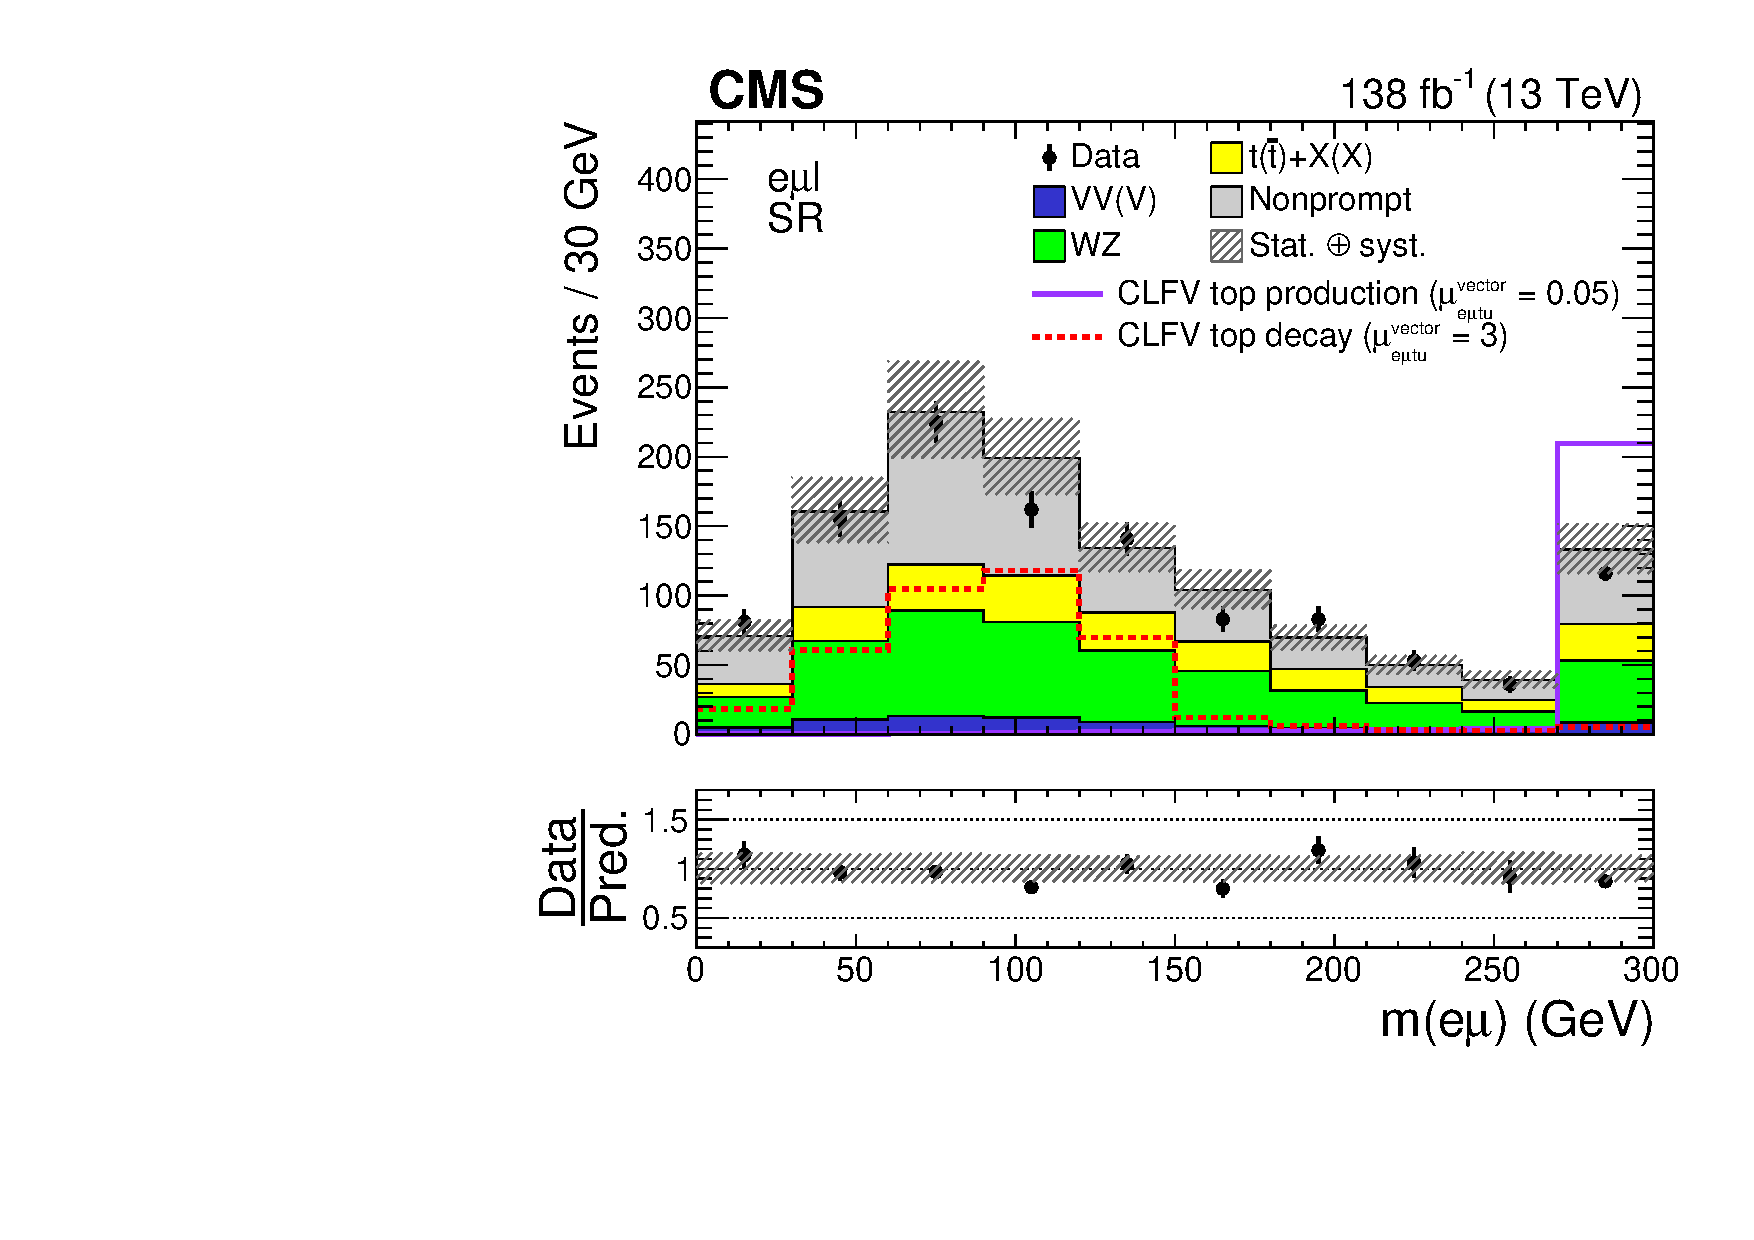
\includegraphics[width=0.45\textwidth]{figures/Part3/Nonprompt/SR/Memu}&
 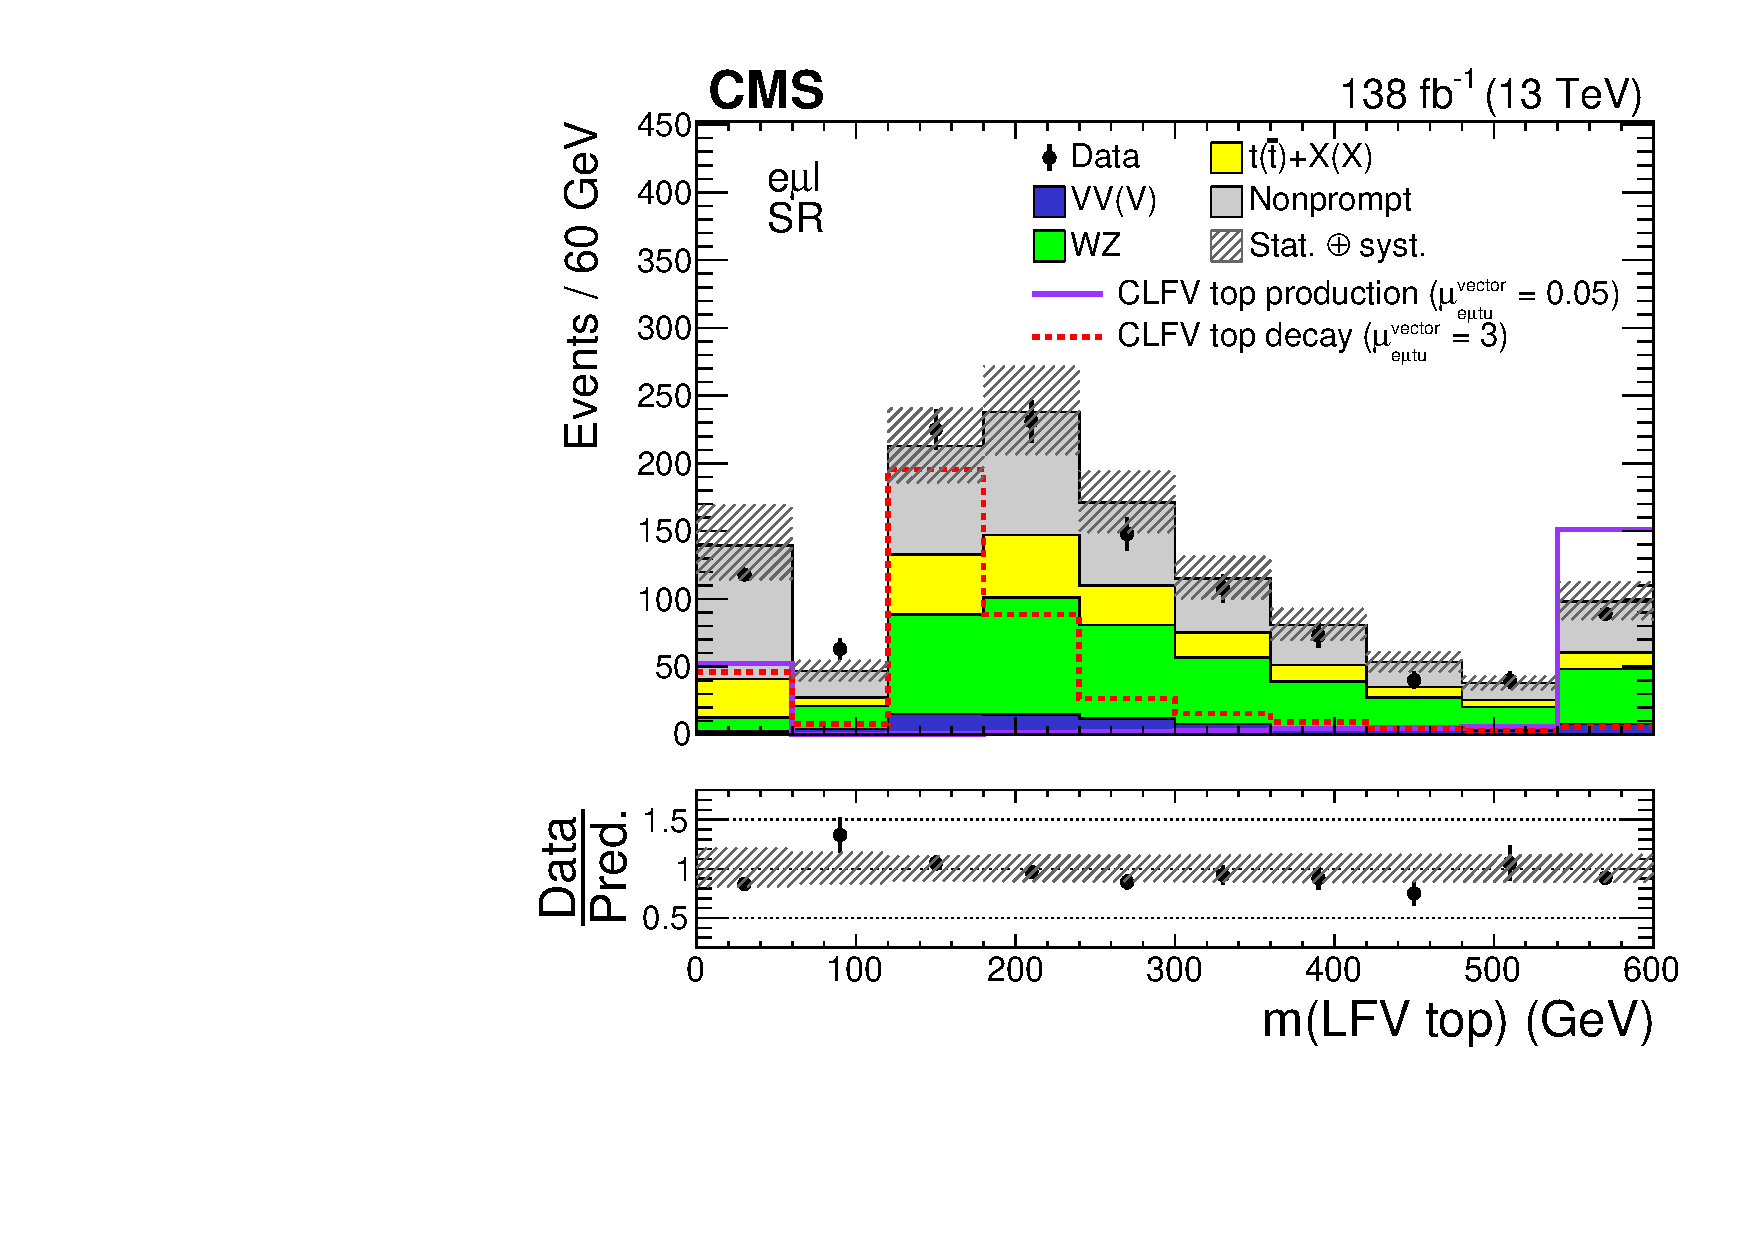
\includegraphics[width=0.45\textwidth]{figures/Part3/Nonprompt/SR/LFVTopmass} \\
 \end{tabular}
 \caption{Distributions of different kinematic variables estimated in SR (full run II). From left to right: b-jet multiplicity, missing transverse energy.}
 \label{fig:SR_DataDriven_1}
 \end{center}
\end{figure}

\begin{figure}[tbh!]
 \begin{center}
 \begin{tabular}{cc}
  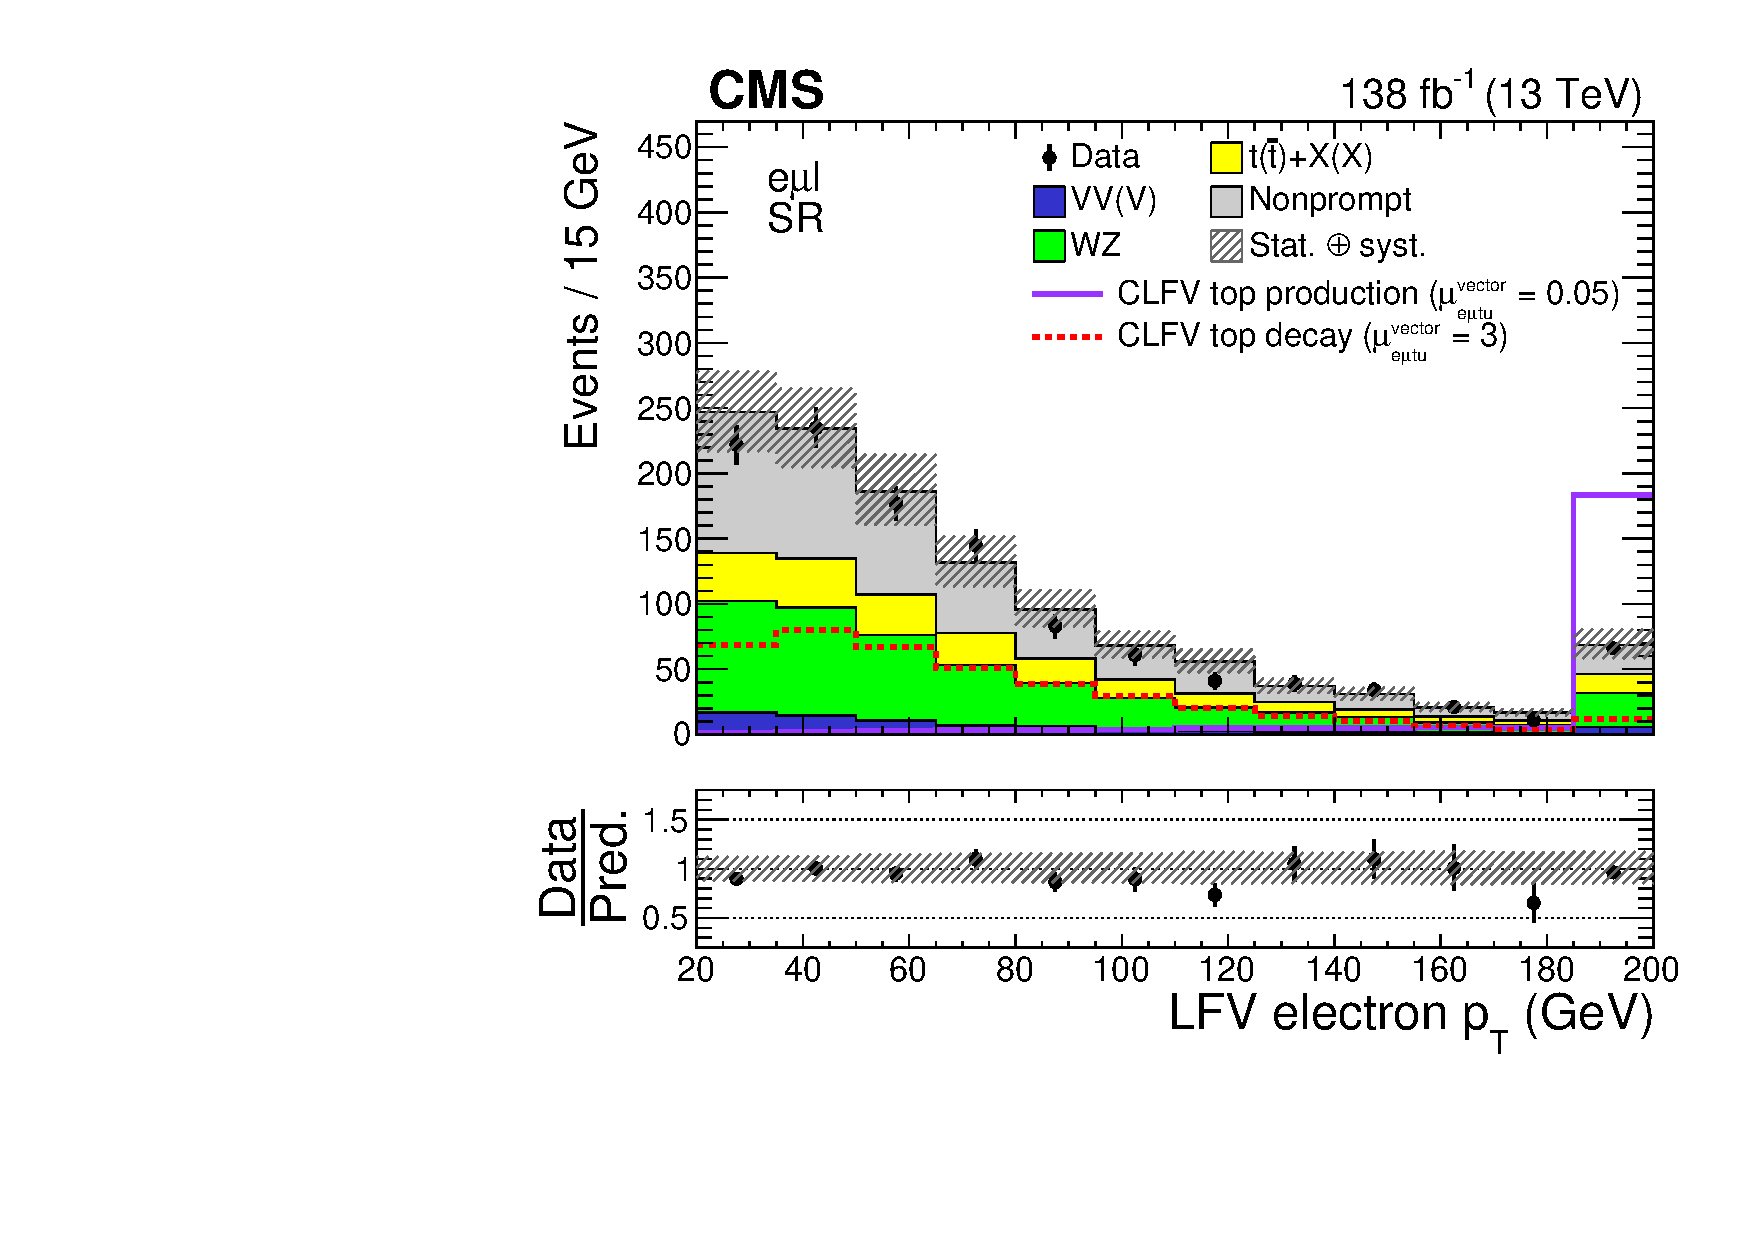
\includegraphics[width=0.45\textwidth]{figures/Part3/Nonprompt/SR/LFVePt}&
 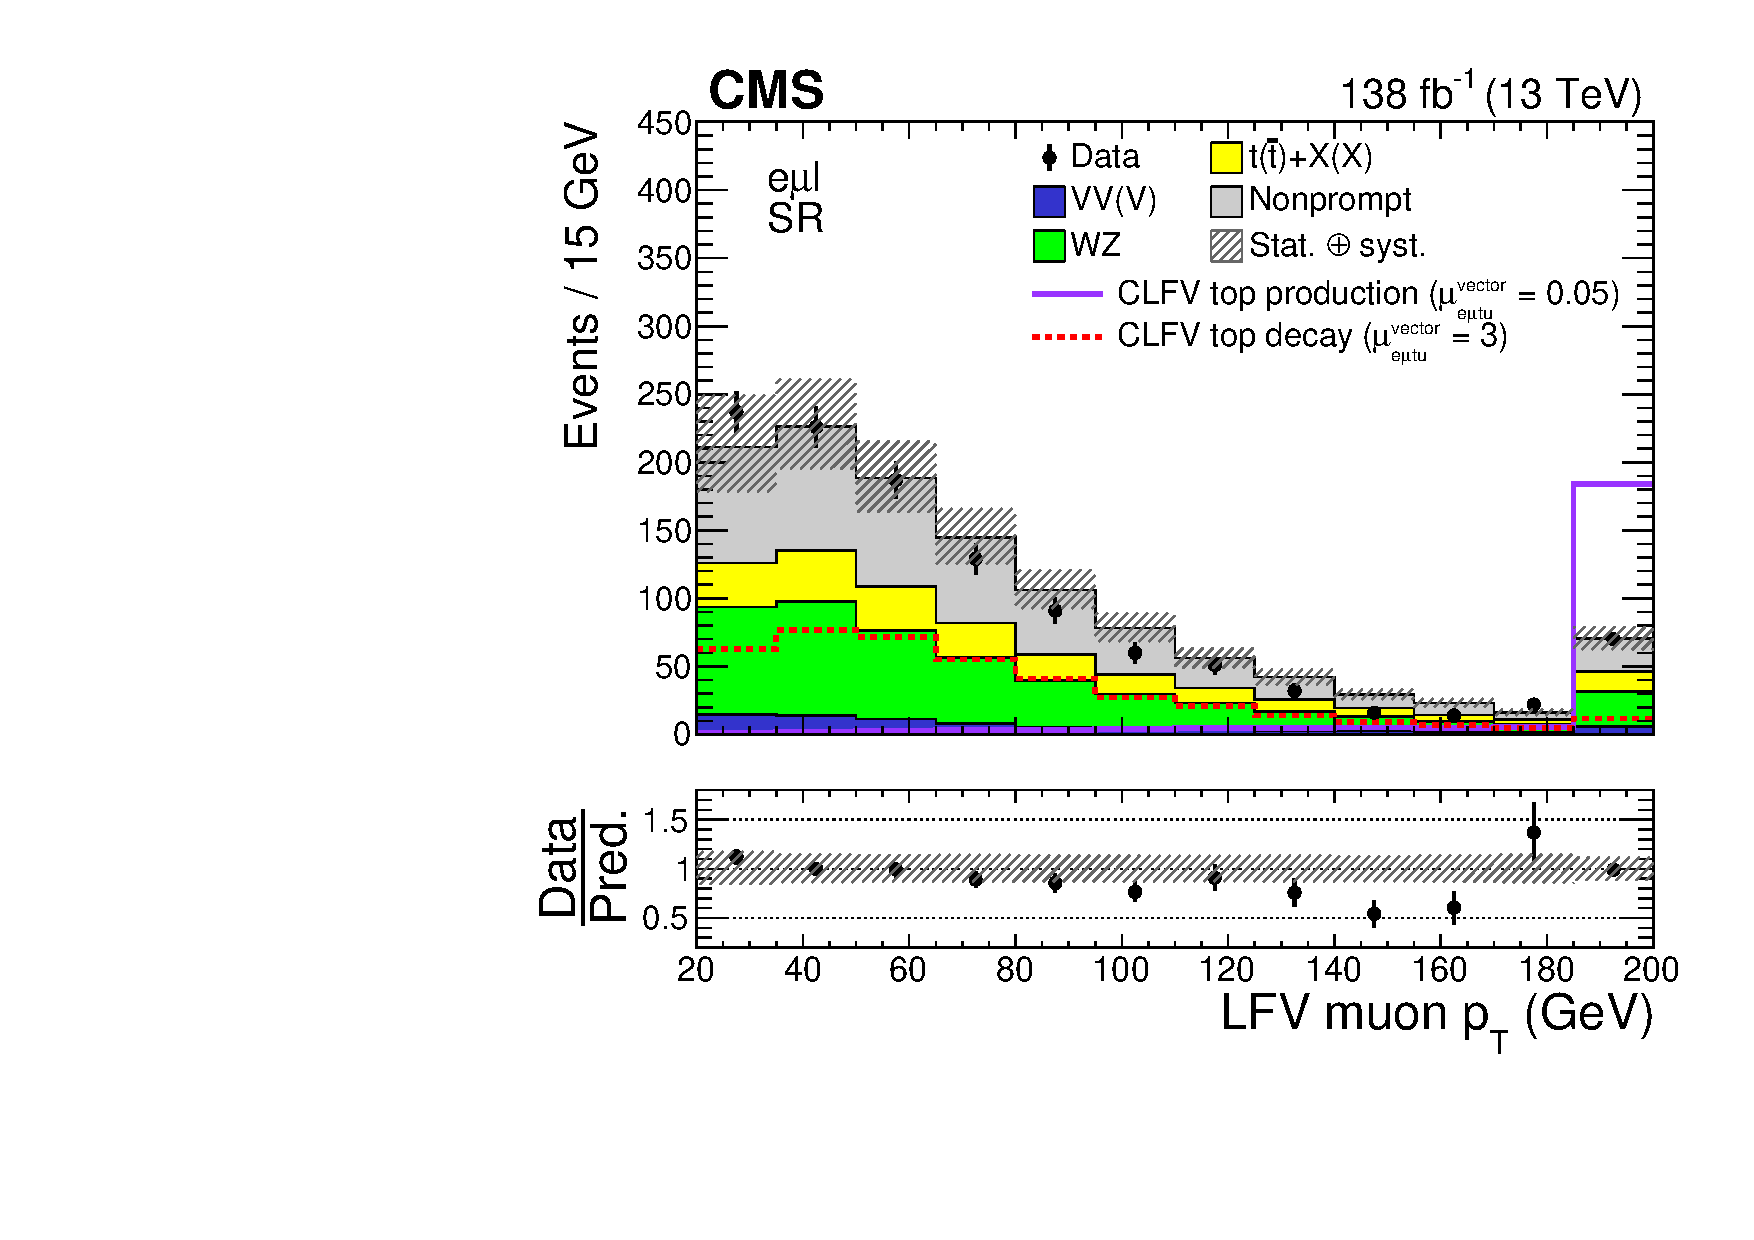
\includegraphics[width=0.45\textwidth]{figures/Part3/Nonprompt/SR/LFVmuPt} \\
 \end{tabular}
 \caption{Distributions of different kinematic variables estimated in SR (full run II). From left to right: b-jet multiplicity, missing transverse energy.}
 \label{fig:SR_DataDriven_2}
 \end{center}
\end{figure}

\begin{figure}[tbh!]
 \begin{center}
 \begin{tabular}{cc}
  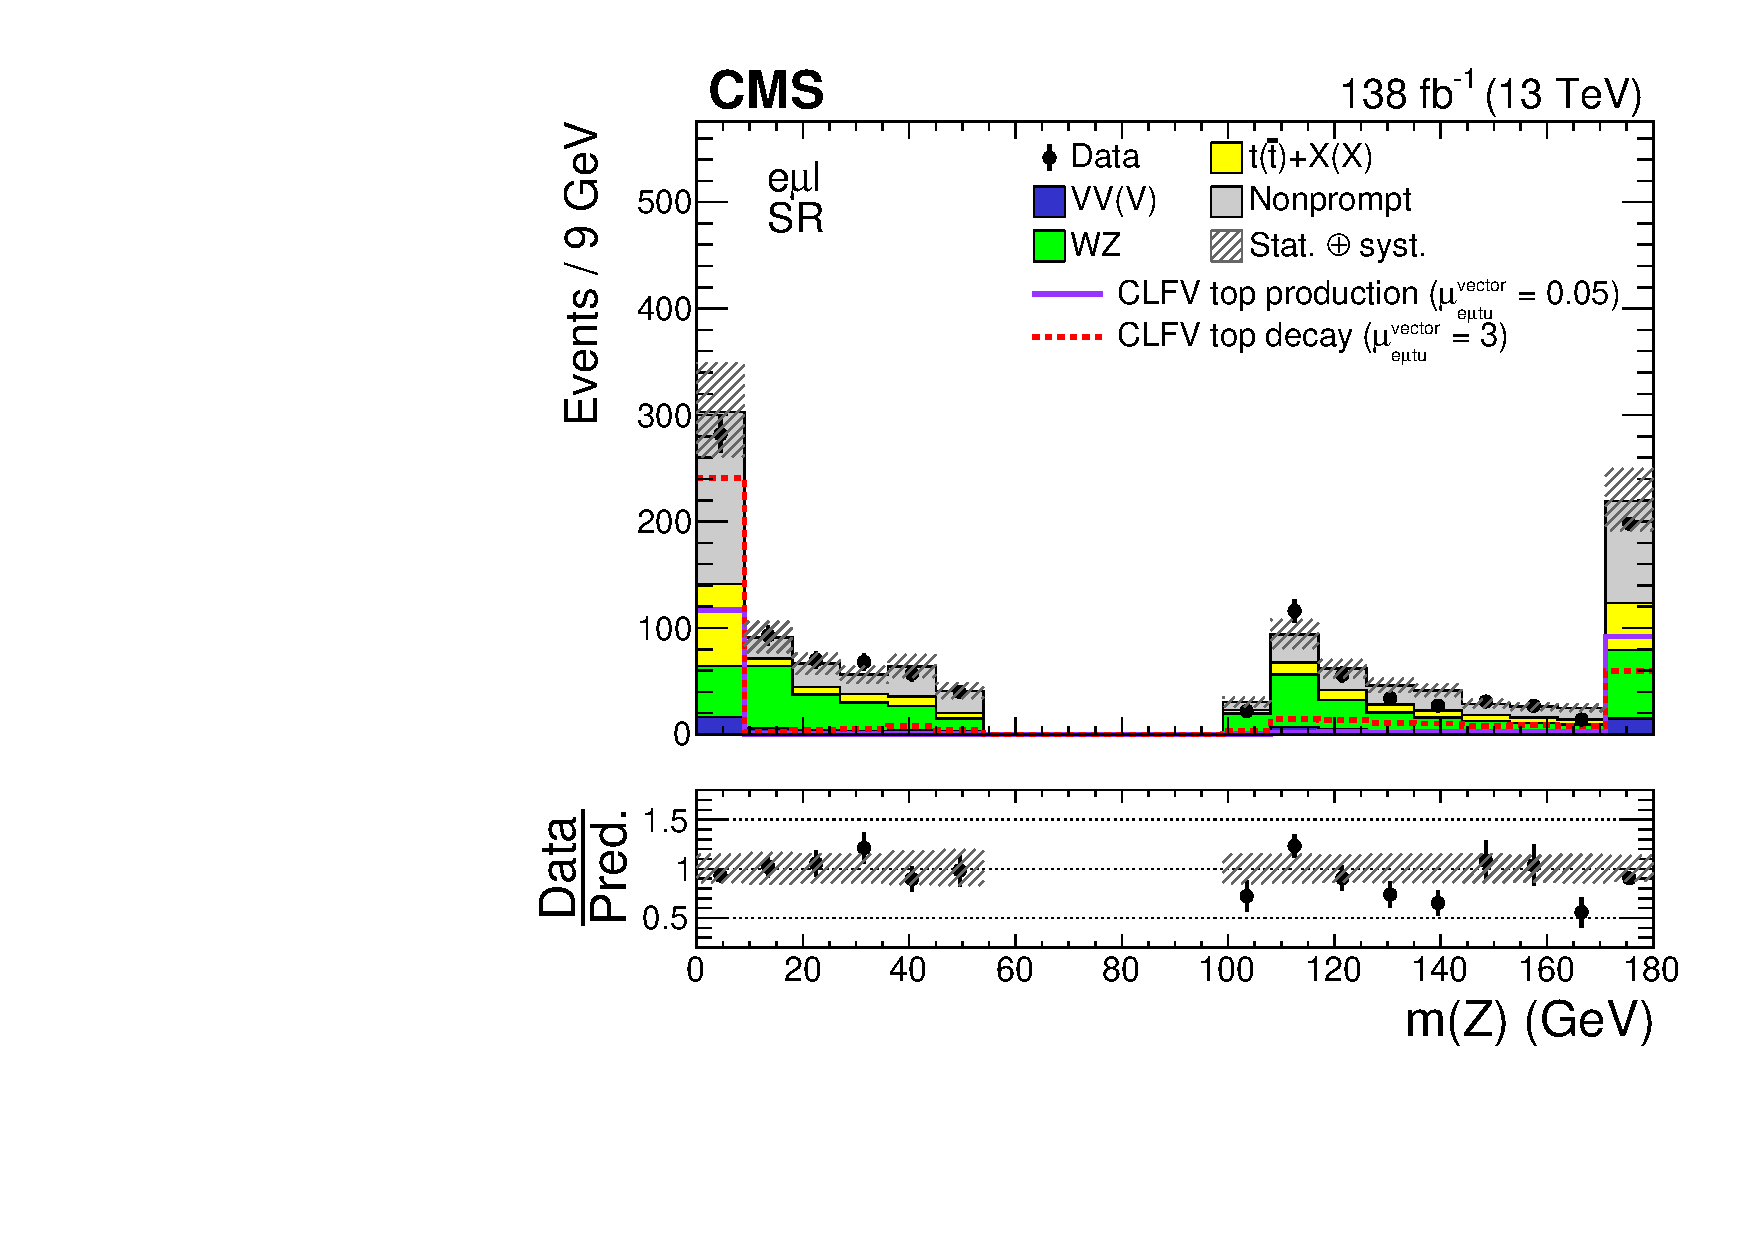
\includegraphics[width=0.45\textwidth]{figures/Part3/Nonprompt/SR/Zmass}&
 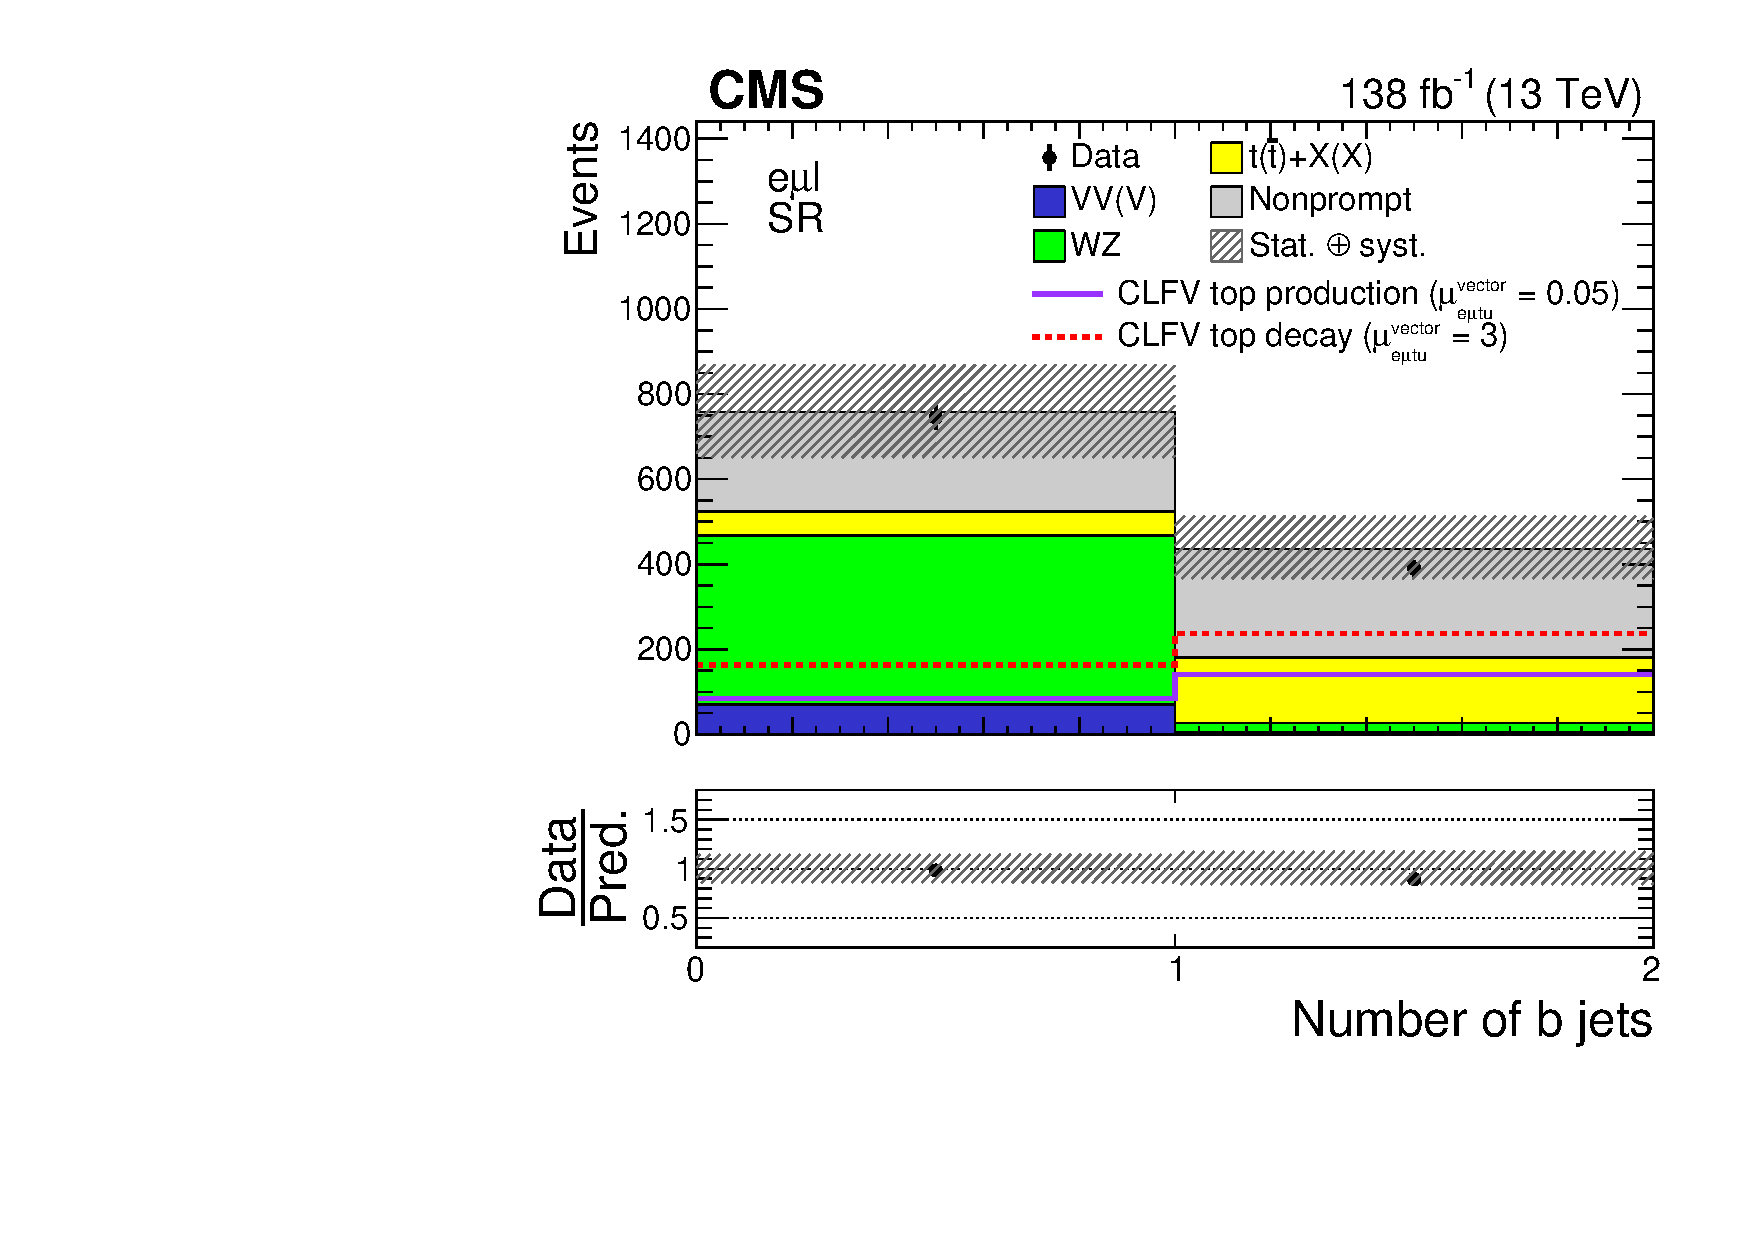
\includegraphics[width=0.45\textwidth]{figures/Part3/Nonprompt/SR/nbjet} \\
 \end{tabular}
 \caption{Distributions of different kinematic variables estimated in SR (full run II). From left to right: mass of the flavor-violating-top-quark candidate, mass of the Z boson candidate}
 \label{fig:SR_DataDriven_3}
 \end{center}
\end{figure}

The number of expected events from various kinds of backgrounds are shown in Table \ref{tab:eventcount}. Representative bin yields and their statistical uncertainties  are summarized in cite{StatError}. 

\begin{table}[th]
\centering
\caption{Expected background contributions and the number of events observed in data collected during 2016--2018. The statistical and systematic uncertainties are added in quadrature. The category ``other backgrounds" includes smaller background contributions containing one or two top quarks plus a boson or quark. The CLFV signal, generated with $C_{e\mu tu}^{\textsf{vector}}/\Lambda^2=1\textsf{TeV}^{-2}$, is also listed for reference. The signal yields include contributions from both top production and decay modes.}
\begin{tabular}{ccc}
\toprule
Process & m(e$\mu$)<150 GeV & m(e$\mu$)>150 GeV \\
\noalign{\vskip 1mm}
\midrule
\noalign{\vskip 1mm}
Nonprompt & $351\pm92$ & $146\pm38$\\
WZ & $275\pm64$ & $145\pm35$\\
ZZ & $33.2\pm6.5$ & $13.1\pm2.6$\\
VVV & $17.0\pm8.5$ & $12.0\pm6.0$\\
ttW & $47.6\pm10.0$ & $40.0\pm9.1$\\
ttZ & $39.1\pm7.9$ & $25.8\pm5.4$\\
ttH & $28.2\pm4.5$ & $10.0\pm1.6$\\
tZq & $5.5\pm1.1$ & $2.5\pm0.5$\\
Other & $7.3\pm3.7$ & $4.5\pm2.3$\\
Total expected & $805\pm123$ & $398\pm57$\\
\noalign{\vskip 1mm}
Data & 783 & 378\\
\noalign{\vskip 1mm}
\midrule
\noalign{\vskip 1mm}
CLFV & 207$\pm$15 & 4440$\pm$215\\
\noalign{\vskip 1mm}
\bottomrule
\end{tabular}
\label{tab:eventcount}
\end{table}

